\documentclass{article}
\usepackage{algorithm}
\usepackage[noend]{algpseudocode}
\usepackage[utf8]{inputenc}
\usepackage[margin=1in]{geometry}
\usepackage{listings}
\usepackage{multicol}
\usepackage{amsmath,amsfonts,graphicx}
\usepackage{fancyhdr}
\usepackage{float}
\usepackage{subfigure}

\makeatletter
\def\BState{\State\hskip-\ALG@thistlm}
\makeatother

\pagestyle{fancy}
\begin{document}



\fancyhf{}
\fancyhead[R]{$\cdot$ \thepage $\cdot$}
\fancyhead[L]{\textit{Yu Hu}}
\fancyhead[C]{Solar ID 110560696}

\begin{center}
{\Large\bf AMS 533 \#1 (Molecular dynamics and minimization)}
\end{center}

\section{Modeling the dynamics of a trapped ion}
(a) With implementation of Forward Euler scheme, $dt=0.01ps$, the plots are presented below.
\begin{eqnarray*}
\mathbf{x}(t+\Delta t) &=& \mathbf{x}(t) + \mathbf{v}(t)\Delta t\\
\mathbf{v}(t+\Delta t) &=& \mathbf{v}(t) + M^{-1}\mathbf{F}(\mathbf{x}(t))\Delta t
\end{eqnarray*}

\begin{figure}[h]
    \centering
    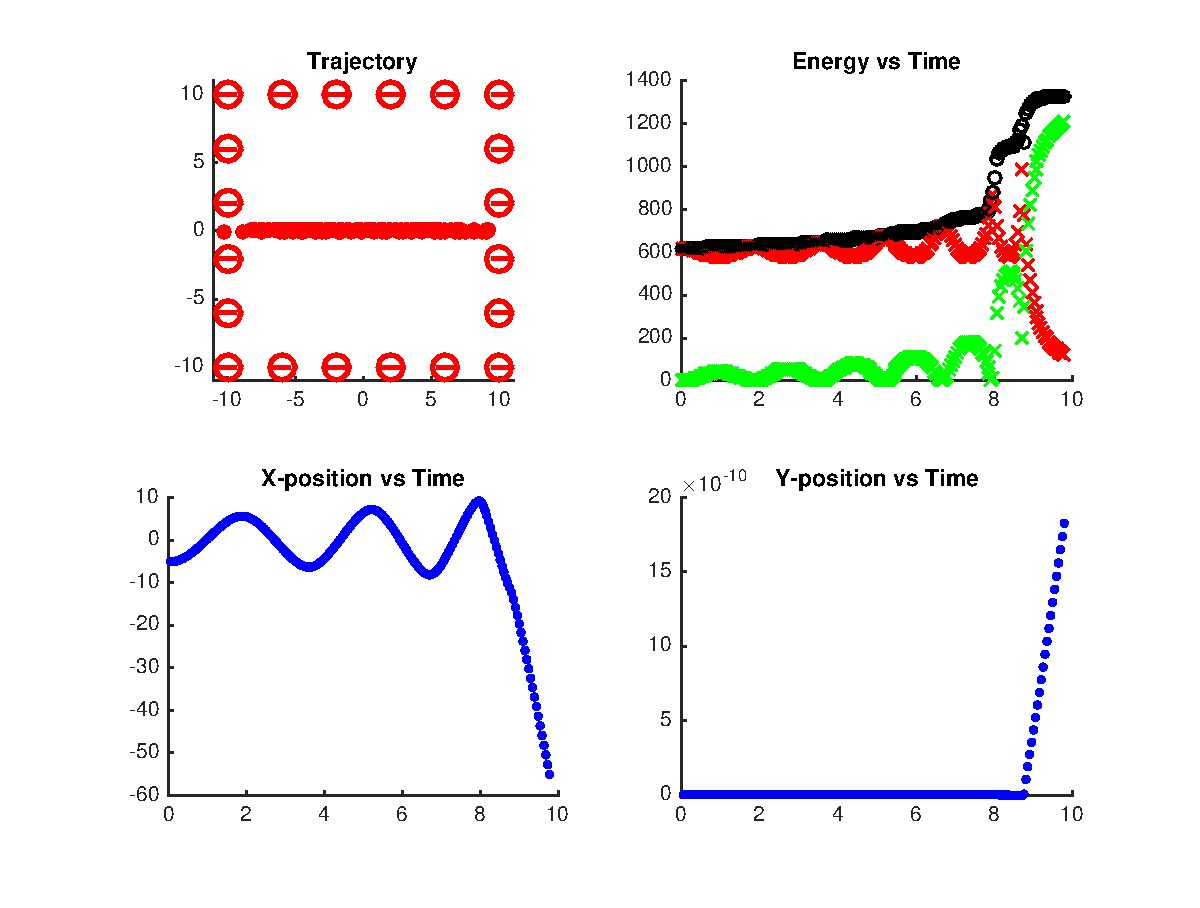
\includegraphics[scale=0.76]{1.eps}
  \end{figure}

\noindent
(b) From the trajectory plot we know that the atom stays on $y=0$ line. The X-position over time plot indicates that the molecule vibrates around the origin point(i.e. back and forth driven by electrostatic and Van der Waals interaction) with increasing magnitude and decreasing periods. 

\vspace{5mm}

\noindent
(c) The kinetic energy $E_k$ and the potential energy develop functions with simple harmonic motion pattern(i.e.sine curves) at beginning, and become unstable after numbers of iterations(from the plot $t>1.6s$). 

Generally $E_k$ minimizes at edge points of oscillation and maximizes at the origin point, while the regulation for $E_{pot}$ follows vice versa. The total energy converges and is stable from the beginning, then deviates largely from conservation later.

\vspace{4mm}
\noindent
(d) $dt=0.001ps$, we see

\begin{center}
{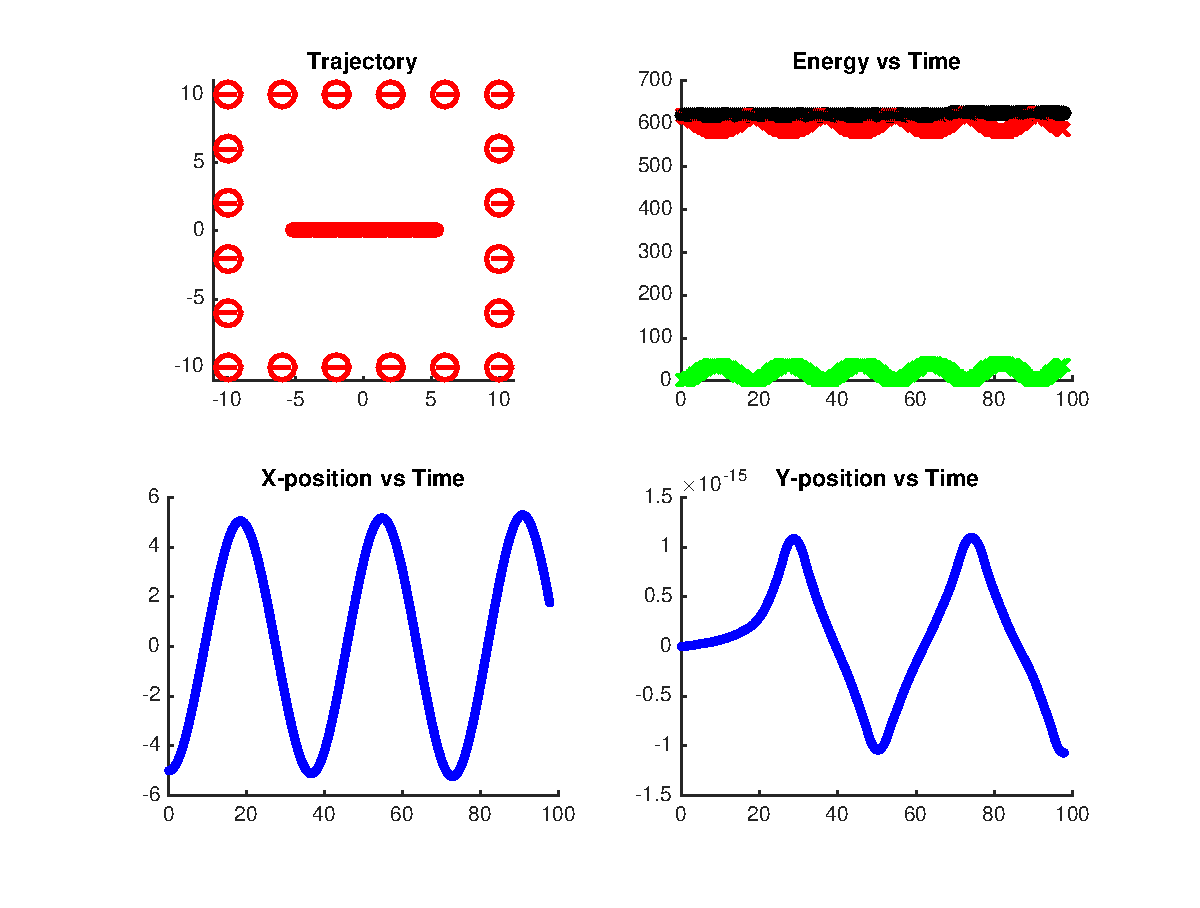
\includegraphics[scale=0.76]{2.eps}}
\end{center}

Apparently we find that the energy $E_{tot} = E_{k} + E_{pot}$ conserves, and both $E_k$ and $E_{pot}$ follow sine curved regulation. Plots of $X$ and $Y$ vs Time indicates that the atom vibrates around origin point with almost stable magnitude on the x-axis.

The error term of position $\mathbf{x}(t)$ of Forward Euler is $\mathcal{O}(t^2)$. By taking smaller time-steps, we made the simulated energy term conserve and avoid energy explosion, for small time-steps depict the functions more precisely at large derivative paragraphs. It also prevents the simulated position from skipping over edge points.

\vspace{4mm}
\noindent
(e) With implication of Velocity Verlet scheme with $dt=0.01ps$, we have
\begin{eqnarray*}
\mathbf{x}(t+\Delta t) &=& \mathbf{x}(t) + \mathbf{v}(t)\Delta t + \frac{1}{2}\mathbf{a}(t)\Delta^2 t\\
\mathbf{v}(t+\Delta t) &=& \mathbf{v}(t) +\frac{1}{2} M^{-1}[\mathbf{F}(\mathbf{x}(t))+\mathbf{F}(\mathbf{x}(t+\Delta t))]\Delta t
\end{eqnarray*}
The trajectory indicates the vibrating motion of the atom conserves at fixed magnitude with Velocity Verlet scheme, while the energetic term $E_{pot}$ begins to vibrate with atomic position $\mathbf{x}(t)$, which results in the vibration of $E_{tot}$ as well. 

The simulated results are more accurate than Forward Euler integration scheme, for the truncation error of Velocity Verlet scheme turns out to be $\mathcal{O}(t^4)$, which is quadratically proportional to Forward Euler.

\vspace{-5mm}
\qquad\quad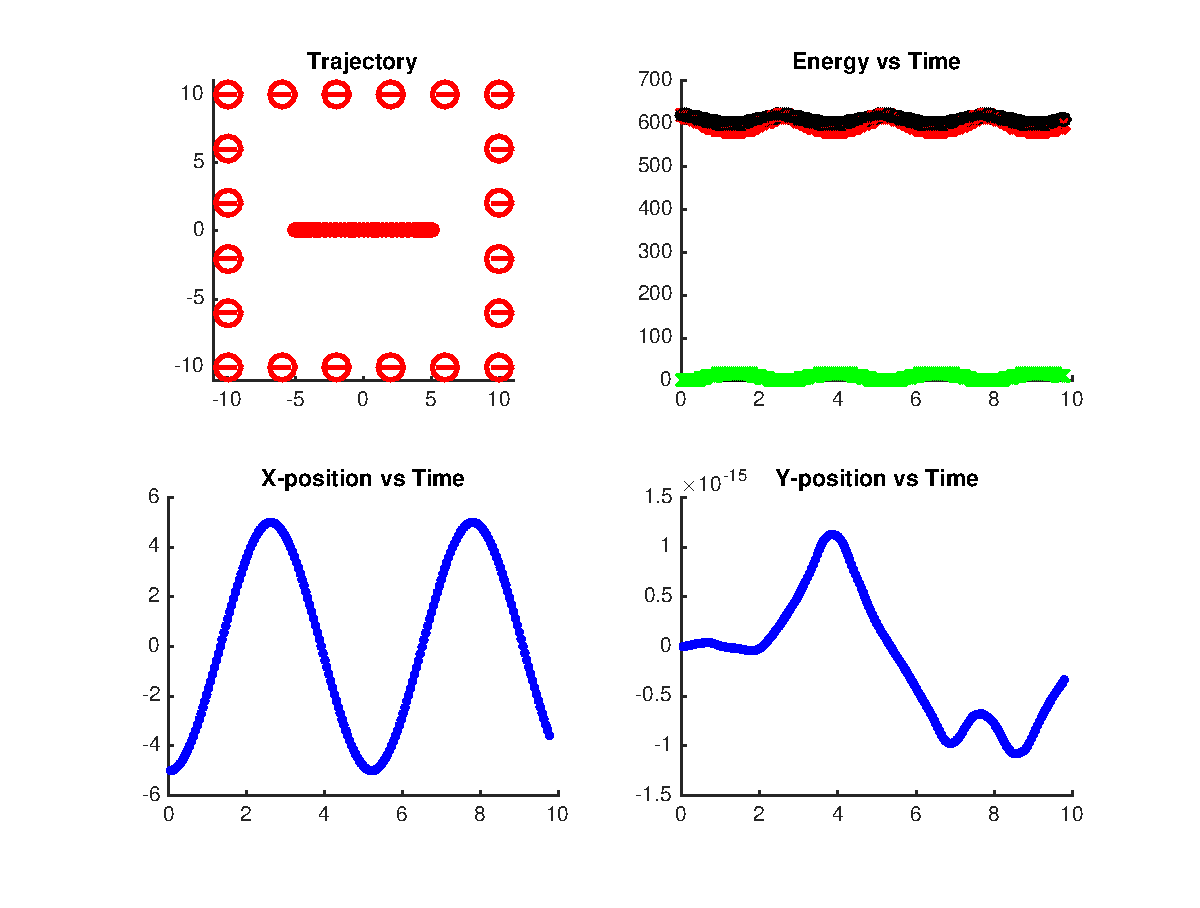
\includegraphics[scale=0.65]{4.eps}


\noindent
(f) Set time step to $dt=0.1ps$, the energy and position terms completely deviated from expected trajectory. According to the $\mathcal{O}(t^2)$ error term, the truncation error of $dt=0.1ps$ case is 100 times of $dt=0.01ps$ and $10^{4}$ times of $dt=0.001ps$.

\qquad\quad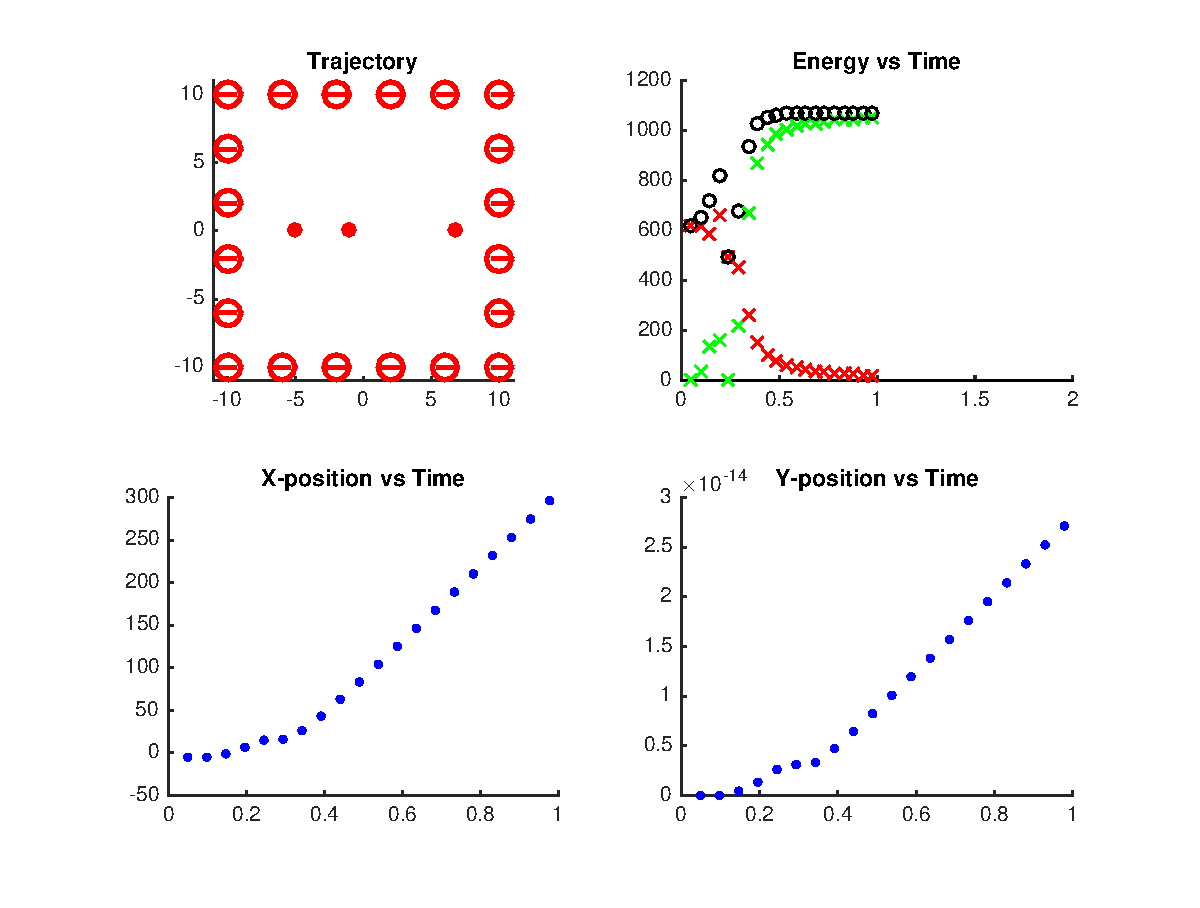
\includegraphics[scale=0.65]{5.eps}

\vspace{6mm}
\noindent
(g) For $\text{Cl}^{-}$ and $\text{Br}^{-}$, we use Velocity Verlet integration scheme with time step $dt=0.001ps$. The upper figure of plots corresponds to $\text{Cl}^{-}$ and the lower to $\text{Br}^{-}$.
\begin{figure}
    \centering
    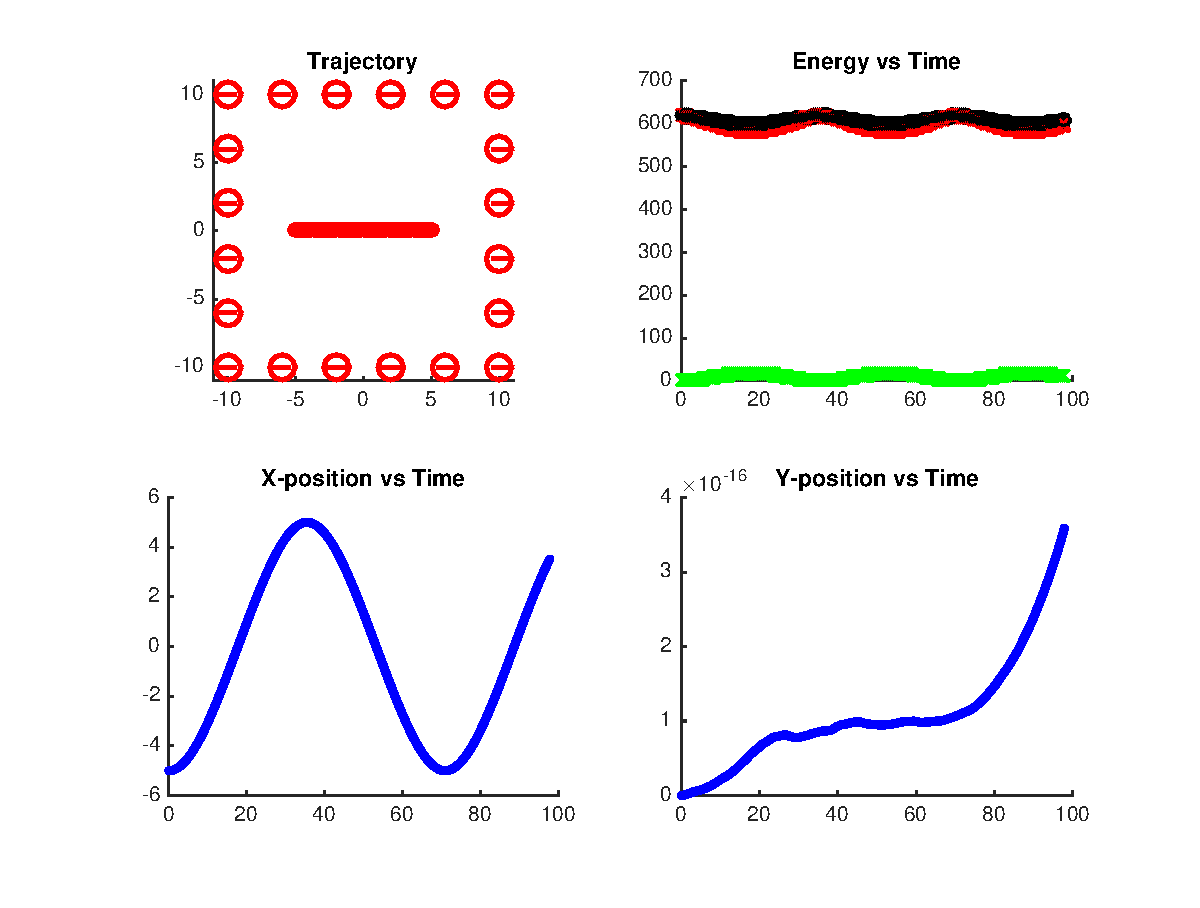
\includegraphics[scale=0.75]{6}
    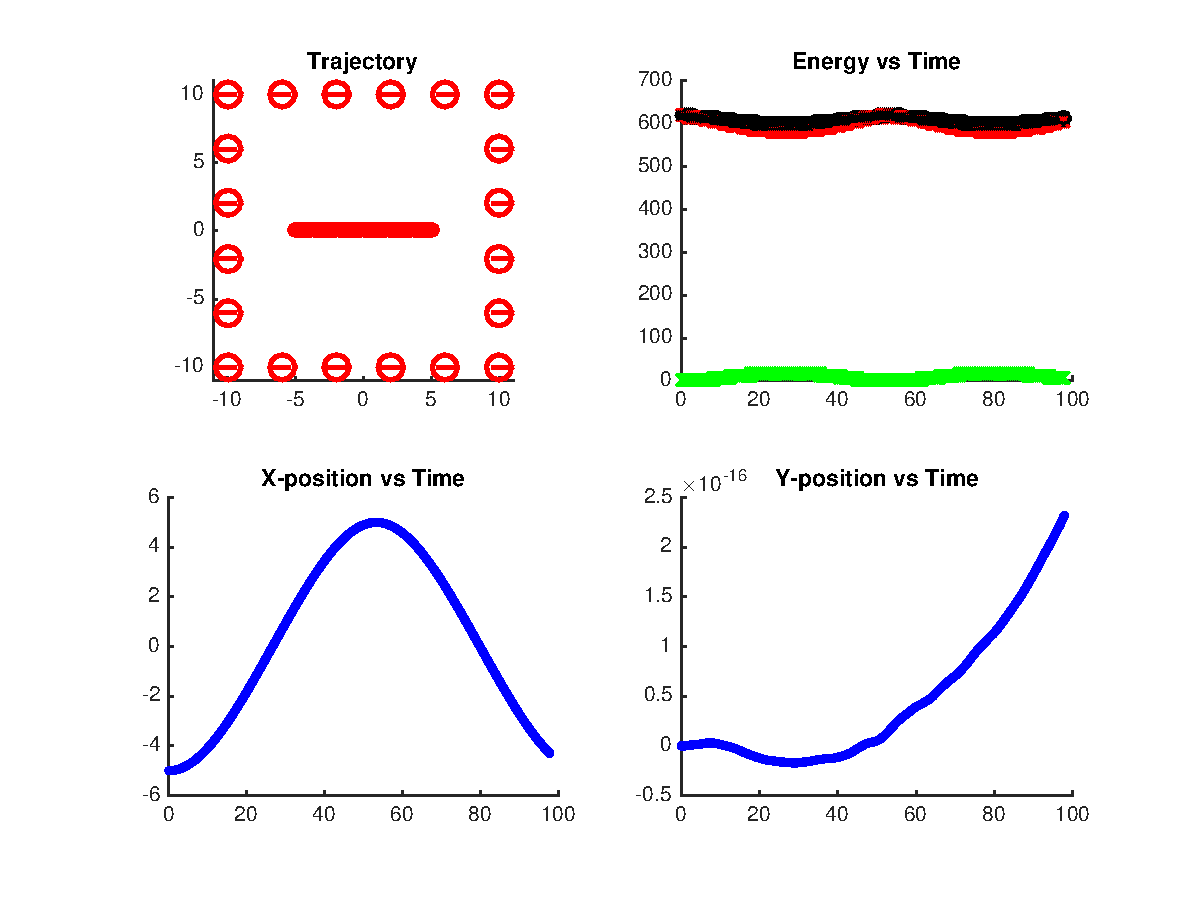
\includegraphics[scale=0.75]{7}
\end{figure}
\newpage
From the two plots of trajectory and $\mathbf{x}(t)$ over time, it is apparent that with changing of atom time, the trajectory persists which indicates that the magnitude does not change. 

The vibrating period increases as atom changes from $\text{F}^{-}$ to $\text{Cl}^{-}$ and then $\text{Br}^{-}$, (i.e. the atomic mass grows), whereas the regulation of energy with position $E(\mathbf{x}(t))$ conserves regardless of atom type.

\vspace{1mm}
\noindent
(h) Set initial position = -9.0\r{A}, the trajectories and energetic terms of $\text{F}^{-}$, $\text{Cl}^{-}$ and $\text{Br}^{-}$ are posted below.

\vspace{-0.5cm}
\begin{figure}[h]
    \centering
    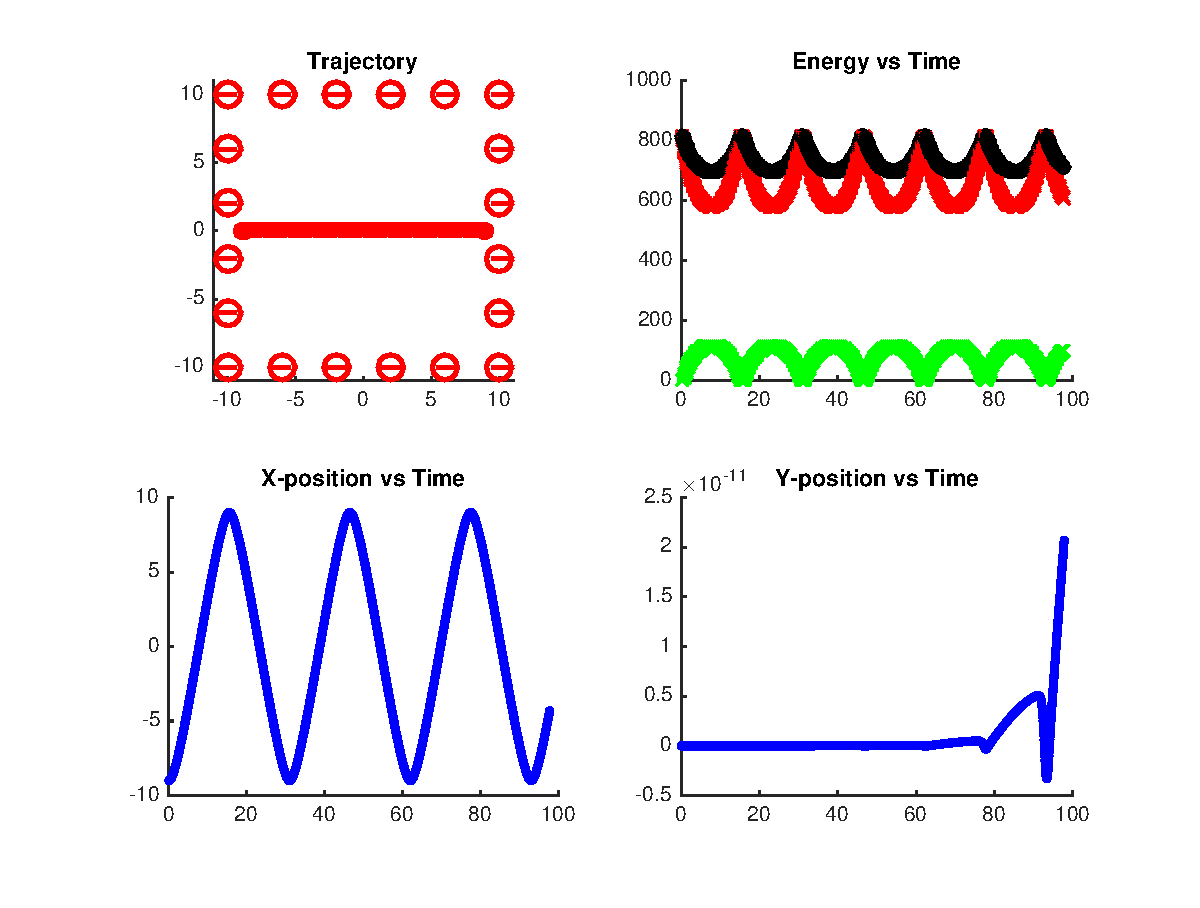
\includegraphics[scale=0.6]{8}
    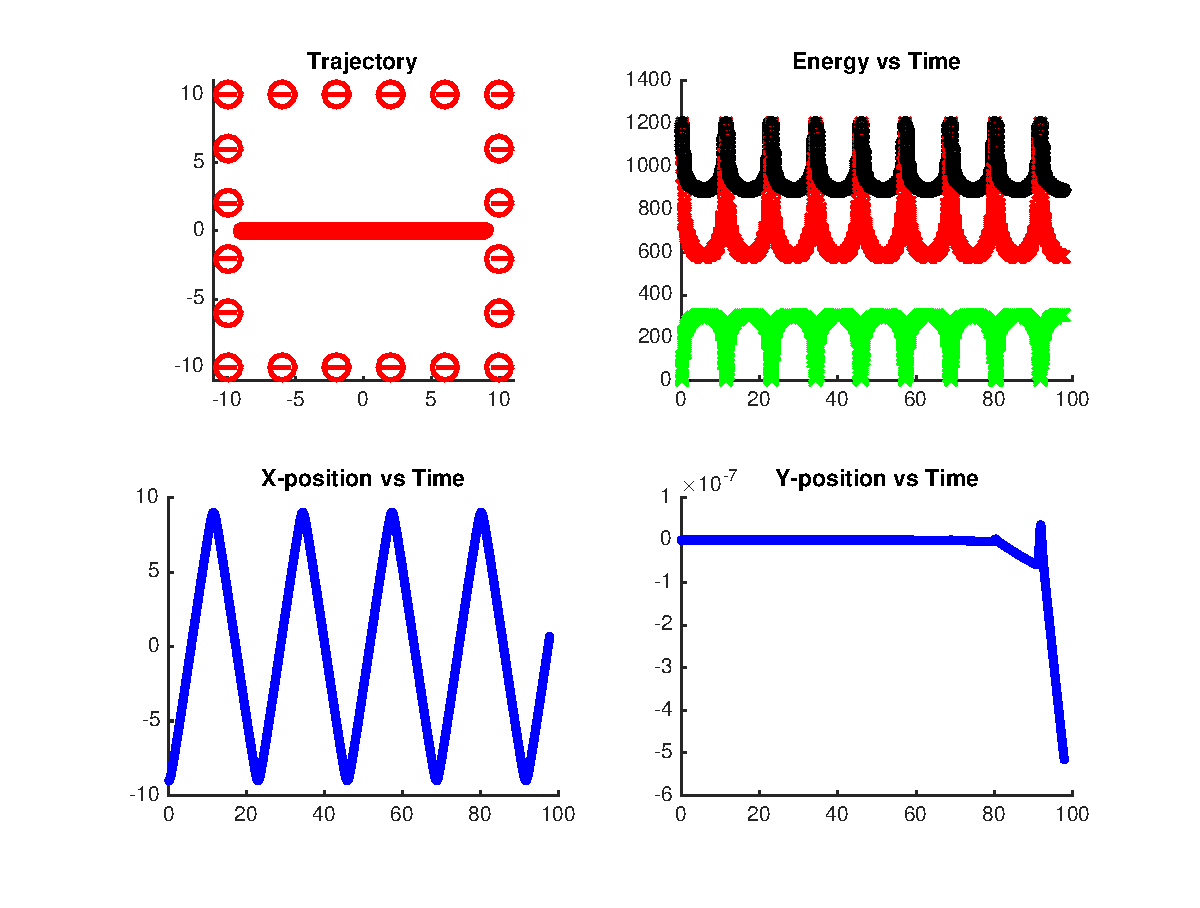
\includegraphics[scale=0.6]{9}
\end{figure}


\begin{figure}[h]
    \centering
    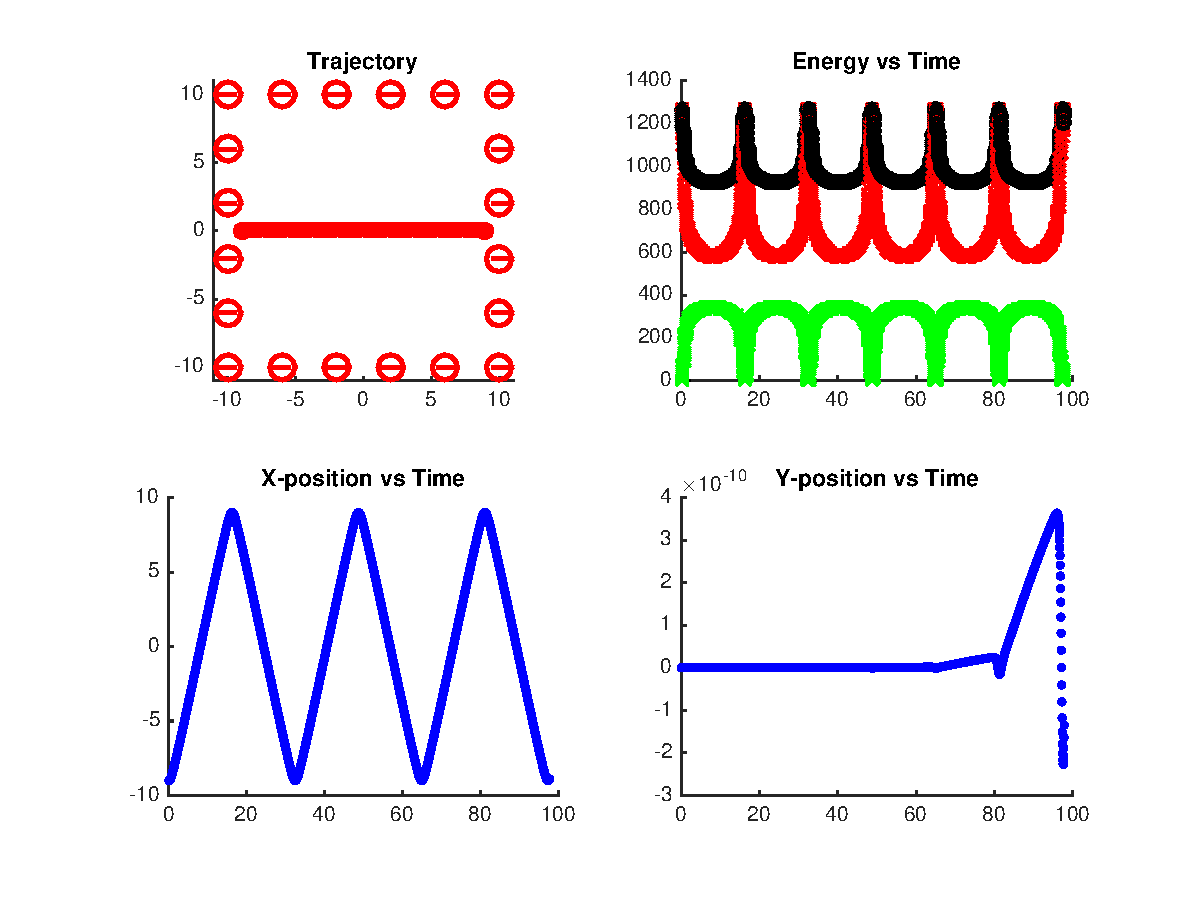
\includegraphics[scale=0.76]{10}
\end{figure}

\vspace{-14mm}

\newpage
\noindent
The trajectories show that the atoms still vibrates around origin point on $x-$axis with fixed magnitude, but the frequency of vibration increased. What is anomaly is that the vibrating frequency of $\text{Cl}^{-}$ tends to be higher than $\text{F}^{-}$ and $\text{Br}^{-}$. One possible reason for these changes is farther initial position yields higher initial $E_{pot}$ and the subsequent steeper descend of it, which amplifies the error at computing derivatives, that is, $\mathbf{x}'(t)$.

For energetic terms, both $E_{pot}$ and $E_{tot}$ vibrates with larger magnitude with position than initial position 5.0\r{A} case. Kinetic energies reach minimum at edge point while potential energies minimize at origin point. Magnitudes of $E_{pot}$ vibration is larger. 

$E_{tot}$ follows vibrating pattern as well, and gets larger magnitude of oscillation with the increasing of atomic weight from $\text{F}^{-}$ to $\text{Br}^{-}$.

\newpage
\section{Finding the minimum energy configuration of a trapped ion}
\textbf{(a)-(b)} We carry out implementation of Steepest Descent(Gradient Descent) minimization scheme with \texttt{convergence= 0.5} and \texttt{maxsteps = 500}, setting initial position randomly in $x,y\in[-10,10]$.
\begin{eqnarray*}
\mathbf{x}_{k+1}&=&\mathbf{x}_{k}+\mathbf{p}~:~ f(\mathbf{x}_{k+1})<f(\mathbf{x}_{k})\\
\mathbf{p}&=&-K\nabla f(\mathbf{x}_{k})
\end{eqnarray*}
At $\textbf{K=1}$ with randomized initial point,$\mathbf{x}_0 = [-3.2456 8.0011]$ 
\begin{figure}[h]
    \centering
    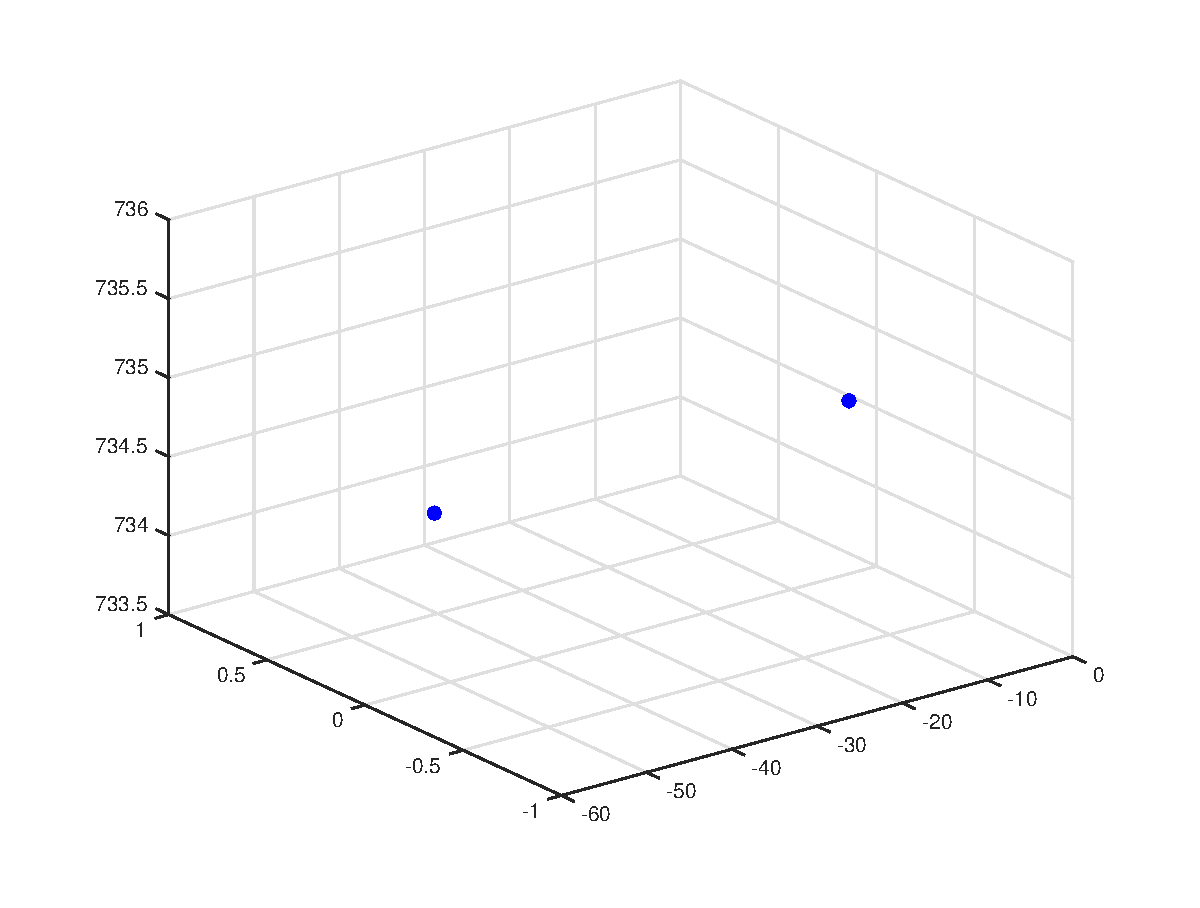
\includegraphics[scale=0.46]{11}
\end{figure}
$$\mathbf{x} = [-51.9796 , -109.917].$$
The simulated result jumps out the boundary and the energy overflows, due to large norm of gradient when $|{\mathbf{x}}|$ is large. So no local minimum has been found.

\noindent
Then we try $\textbf{K=0.5}$, with randomization $\mathbf{x}_0 = [-2.6151 -7.7759]$,
\begin{figure}[h]
    \centering
    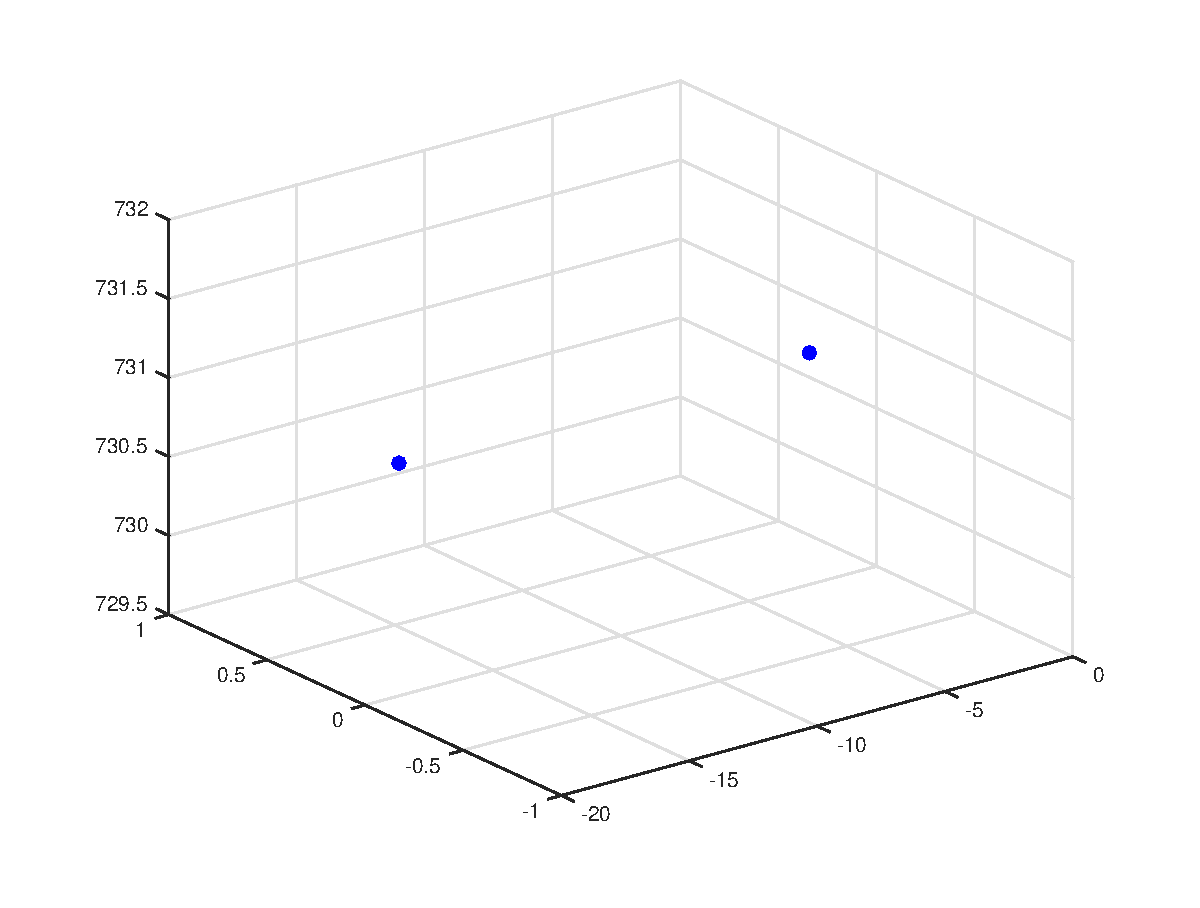
\includegraphics[scale=0.46]{12}
\end{figure}
$$\mathbf{x} = [-18.70 , 69.8404],~E(\mathbf{x}) = 730.9684.$$
Out-ranged result position generated by simulation, no local minimum found.

Try another simulation with $\mathbf{x}_0 = [5.6050,-2.2052]$
\begin{figure}[h]
    \centering
    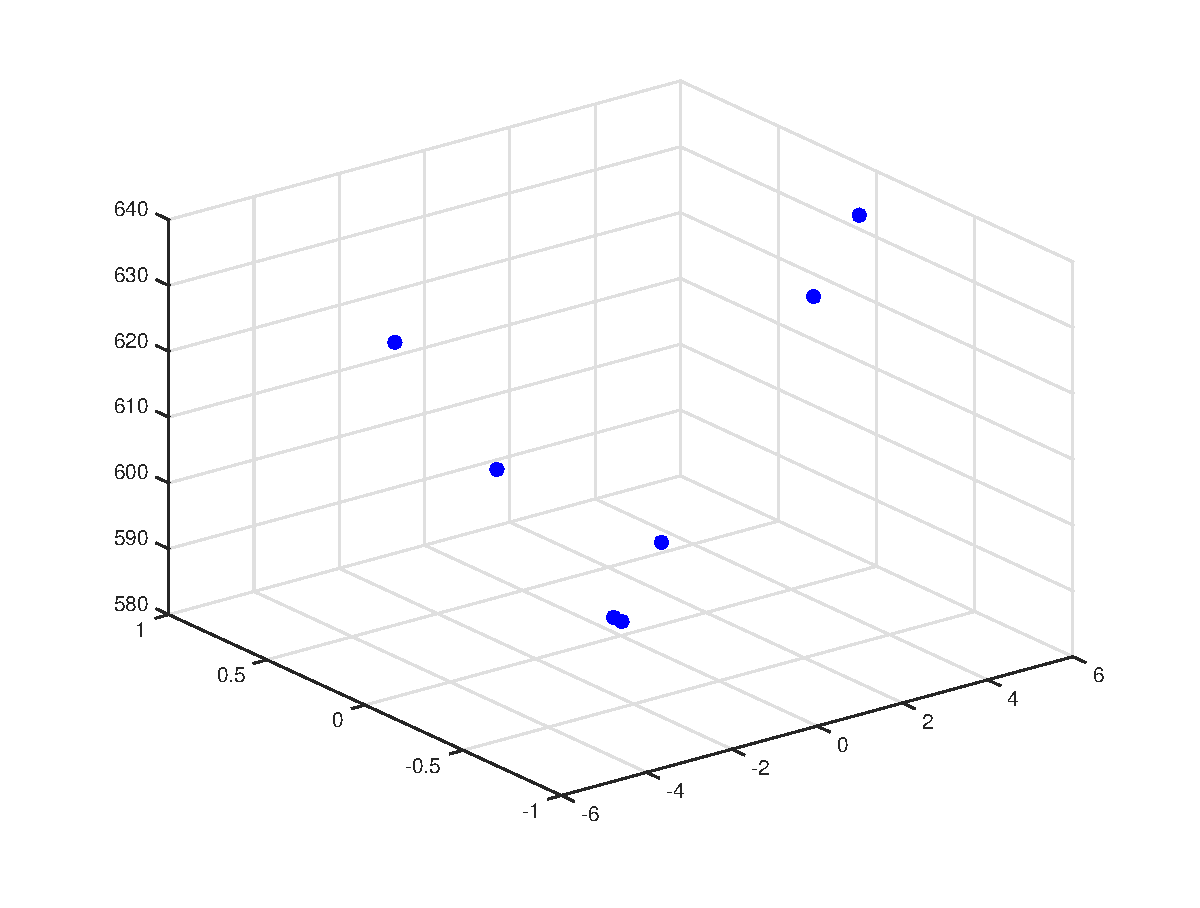
\includegraphics[scale=0.46]{13}
\end{figure}
$$\mathbf{x} = [0.0281,0.0],~E(\mathbf{x}) = 582.0627,~\text{Step}~k = 7.$$
The outcome converges to the origin point, which is consistent with analytical calculation. Thus $K=0.5$ \textbf{could not guarantee a local minimum for all initial points} $x,y\in[-10,10]$, especially if $|\mathbf{x}_i|(i\in\{1,2\})$ is apparently large.

\vspace{2mm}
\noindent
For a \textbf{much smaller $K$, for instance $K = 0.05~\text{or} ~0.01$}, it enlarges the gradient convergence range for initial position rapidly, but still generates out-ranged results when $x$ or $y$ is significantly large. 

\noindent
See the figures below for $K = 0.05, \mathbf{x}_{10} = [0.9402,-4.0736]~\text{and}~\mathbf{x}_{20} = [4.8939,-6.2209]$.
\begin{figure}[h]
    \centering
    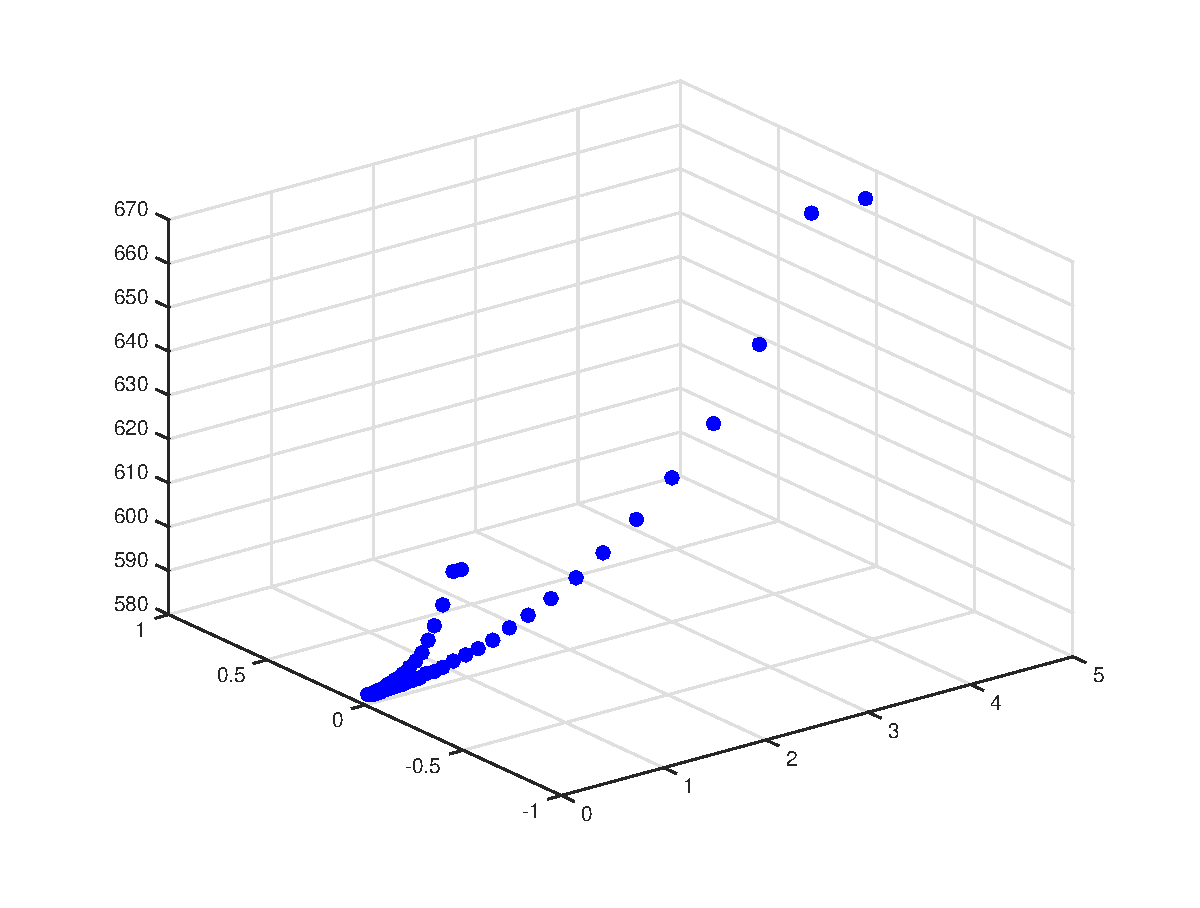
\includegraphics[scale=0.46]{14}
\end{figure}
\begin{eqnarray*}
\mathbf{x}_{1} &=& [0.0607,-0.2050], E(\mathbf{x}_1) = 582.1149, k_1 = 24\\
\mathbf{x}_{2} &=& [0.1353,-0.1435], E(\mathbf{x}_2) = 582.1069, k_2 = 30
\end{eqnarray*}

And $K = 0.01$, initial positions $\mathbf{x}_{10} = [3.7355,-6.3298]~\text{and}~\mathbf{x}_{20} = [-2.493,8.8615]$.

\begin{figure}[h]
    \centering
    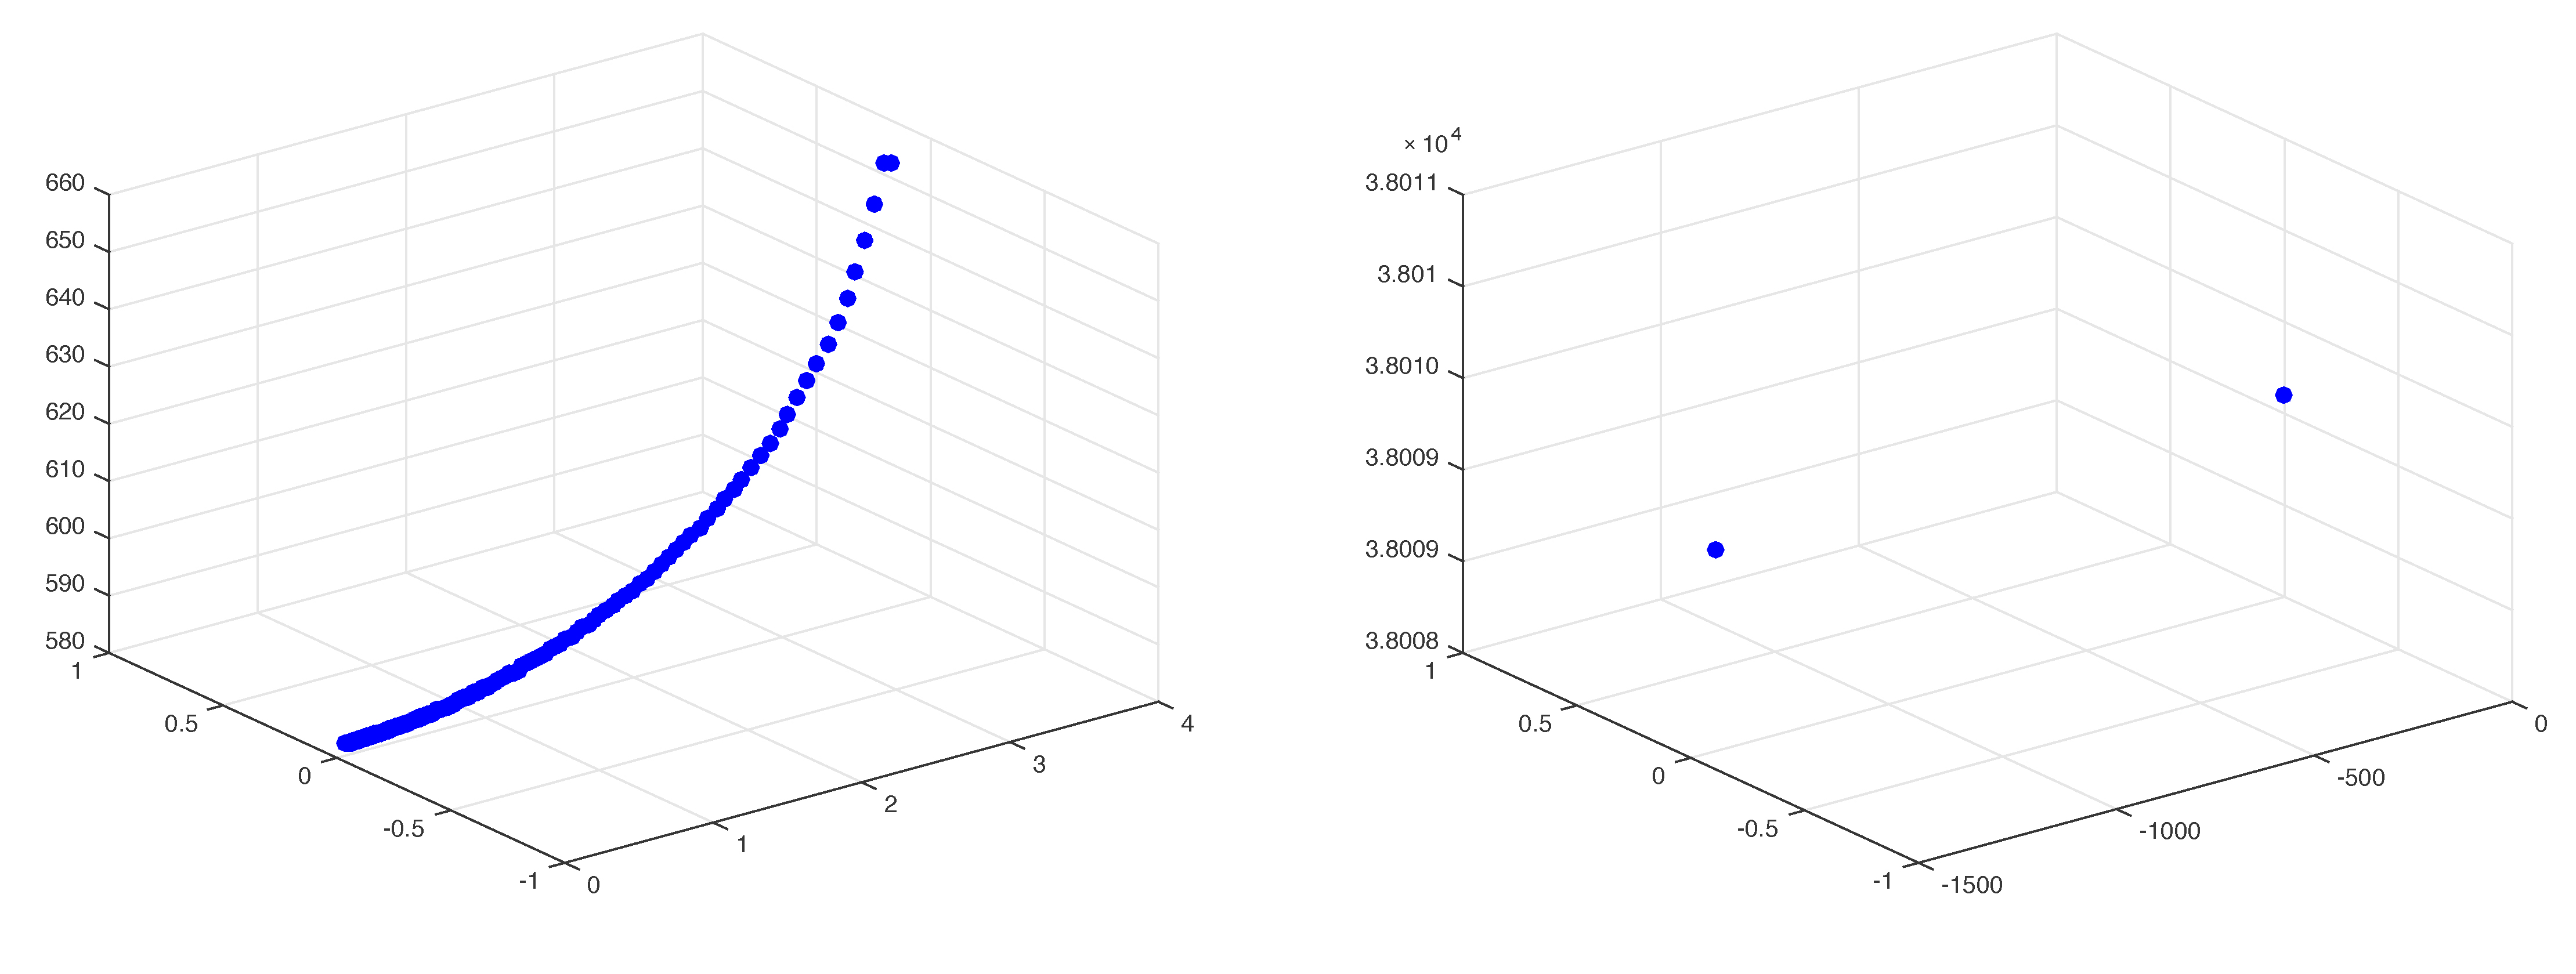
\includegraphics[scale=0.42]{15.jpg}
\end{figure}
\newpage
\begin{eqnarray*}
\mathbf{x}_{1} &=& [0.1313,-0.1651], E(\mathbf{x}_1) = 582.113, k_1 = 147\\
\mathbf{x}_{2} &:& \text{Runs out of range, no local minimum}.
\end{eqnarray*}

\vspace{3mm}
\noindent
\textbf{(c)} We change the convergence threshold from 0.5 to 0.2, and retry those simulations in (a) and (b).

\vspace{2mm}

$K=1$, initial position $\mathbf{x}_0 = [5.6045,-8.3775]$, result jumps outside the range, no feasible local minimum.


$K=0.5$, initial position $\mathbf{x}_0 = [8.5877,5.5143]$, result out-ranged, no feasible local minimum.

\begin{figure}[h]
\begin{minipage}[t]{0.5\linewidth}
\centering
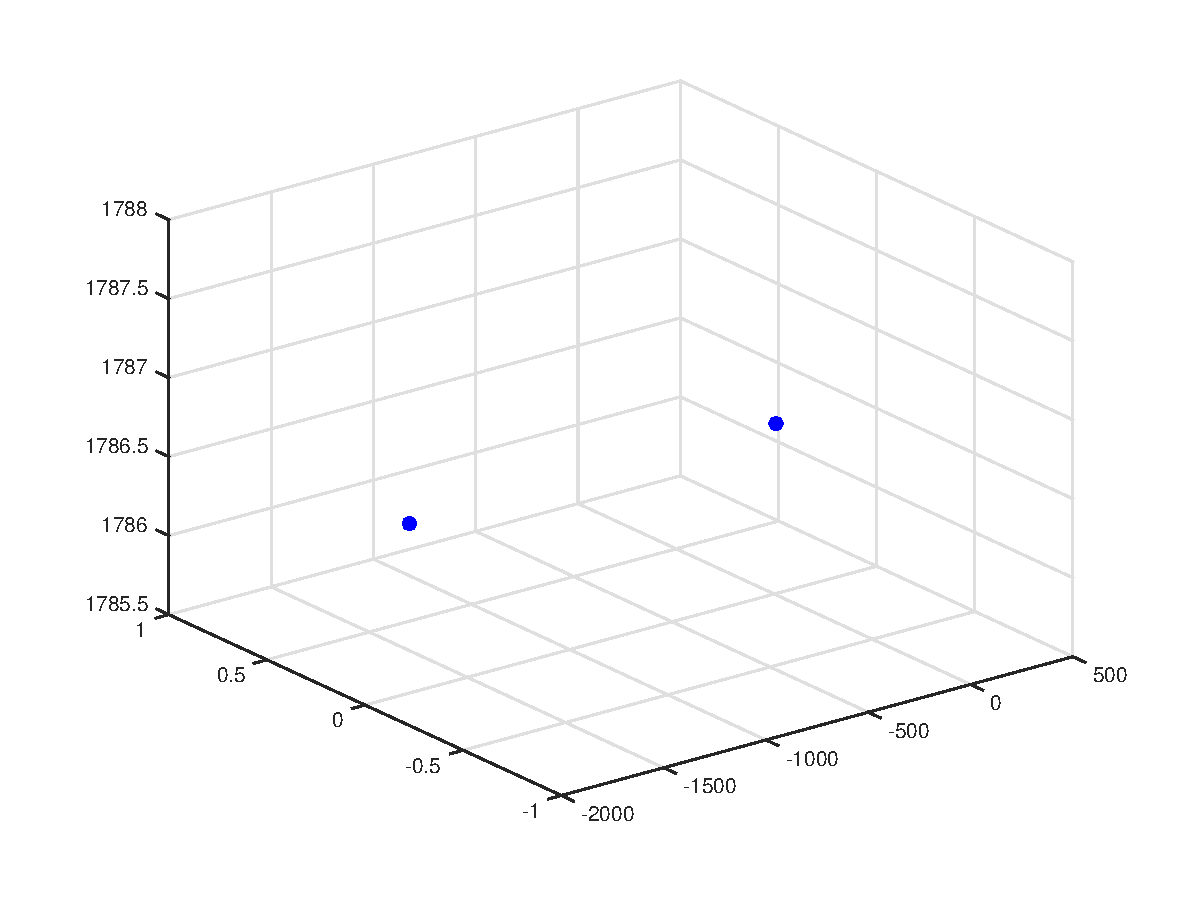
\includegraphics[scale=0.4]{16}
\caption{$K=1$}
\end{minipage}%
\begin{minipage}[t]{0.5\linewidth}
\centering
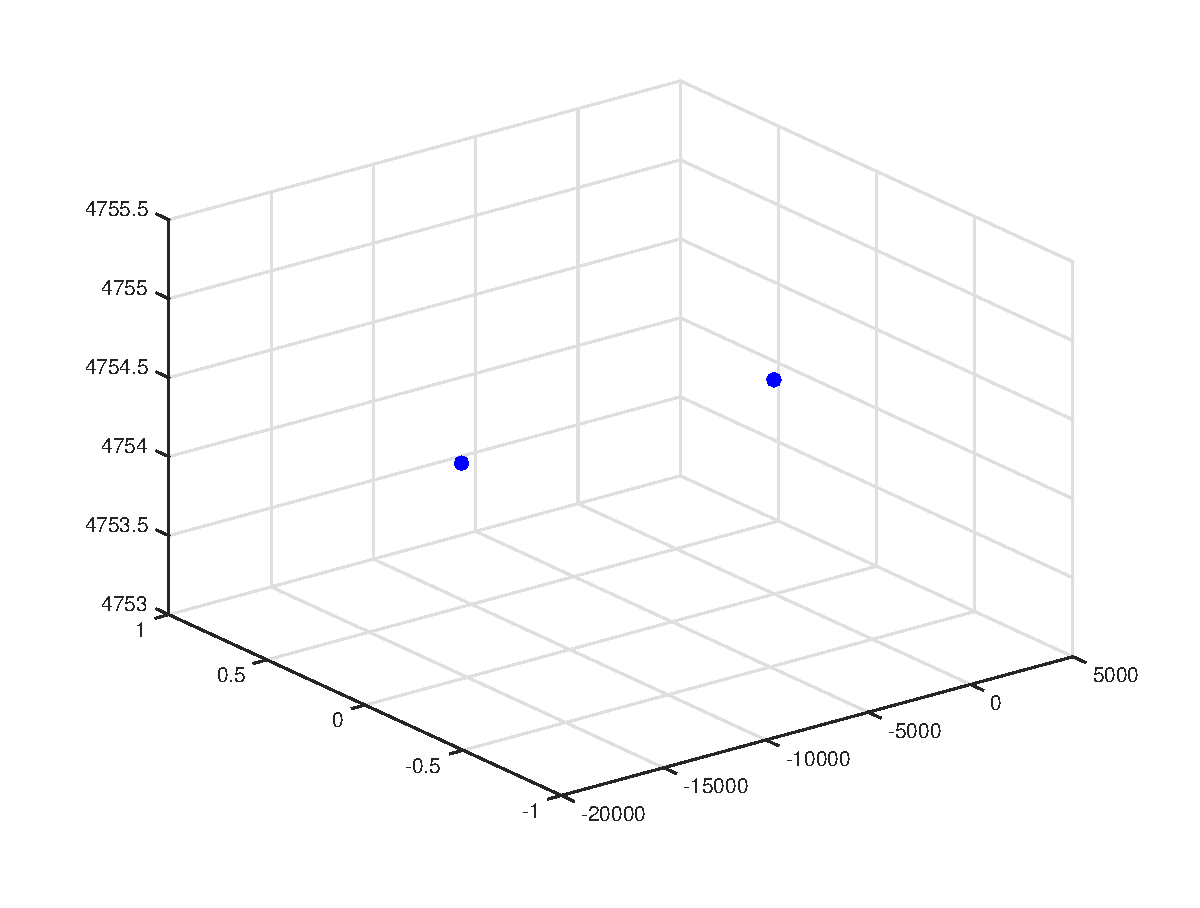
\includegraphics[scale=0.4]{17}
\caption{$K=0.5$}
\end{minipage}
\end{figure}

\noindent
For \textbf{initial positions close enough to $O$} and \textbf{small enough $K$}, which could yield convergence, switching $\epsilon$ from 0.5 to 0.2 yields feasible result closer to $O$, with lower energy as well. 

\vspace{2mm}
$K=0.5$, initial position $\mathbf{x}_{10} = [-1.0643,-3.8730]$, and $K=0.2$, initial position $\mathbf{x}_{20} = [6.3526, 5.8966]$.


\begin{figure}[h]
\begin{minipage}[t]{0.5\linewidth}
\centering
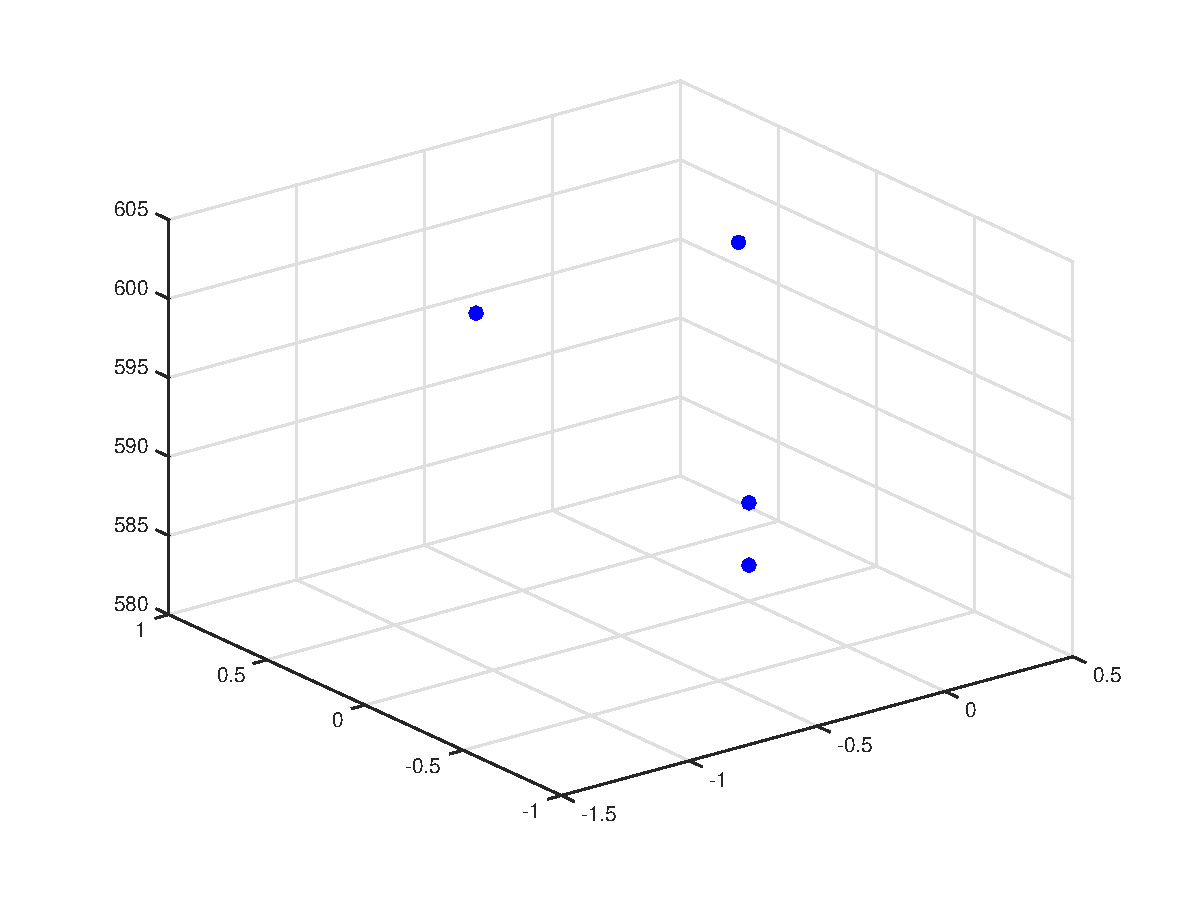
\includegraphics[scale=0.4]{18}
\caption{$K=0.5,\mathbf{x}_1$}
\end{minipage}%
\begin{minipage}[t]{0.5\linewidth}
\centering
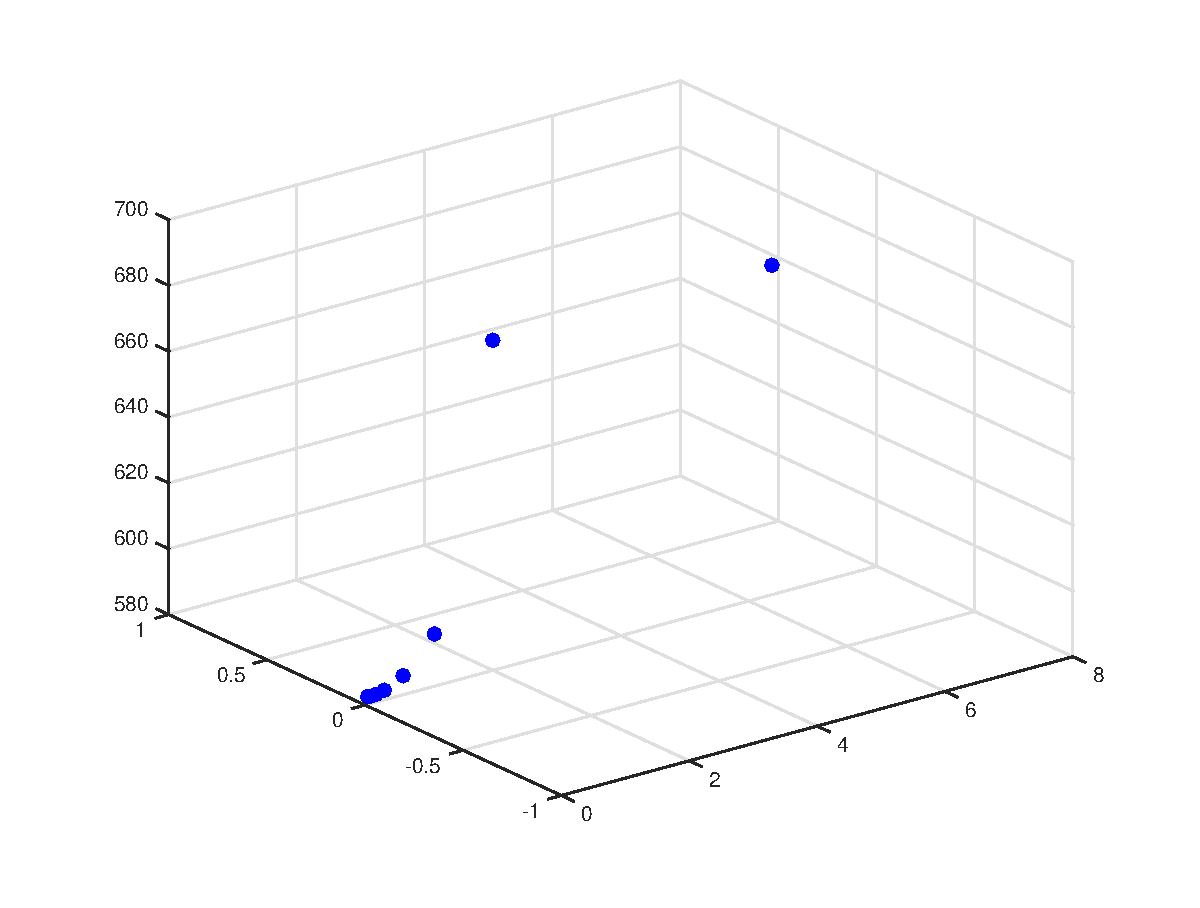
\includegraphics[scale=0.4]{19}
\caption{$K=0.2,\mathbf{x}_2$}
\end{minipage}
\end{figure}
\begin{eqnarray*}
\mathbf{x}_{1} &= [-0.000673,0.0696], ~E(\mathbf{x}_1) =& 582.0674, ~k_1 = 4\\
\mathbf{x}_{2} &= [~0.048540,0.0593], ~E(\mathbf{x}_2) =& 582.0686, ~k_2 = 8
\end{eqnarray*}
\noindent
For \textbf{even smaller $K$}, there is still \textbf{no guarantee for feasible results near margin of the system}, whereas all {feasible results are optimized} than $\epsilon = 0.5$ situation.

\newpage
$K=0.05$, initial position $\mathbf{x}_{30} = [2.3718,-2.5944]$, and $K=0.01$, initial position $\mathbf{x}_{40} = [6.2316 0.6565]$.

$K=0.01$, initial position $\mathbf{x}_{50} = [9.0501,-3.4418]$.

\begin{figure}[h]
\begin{minipage}[t]{0.5\linewidth}
\centering
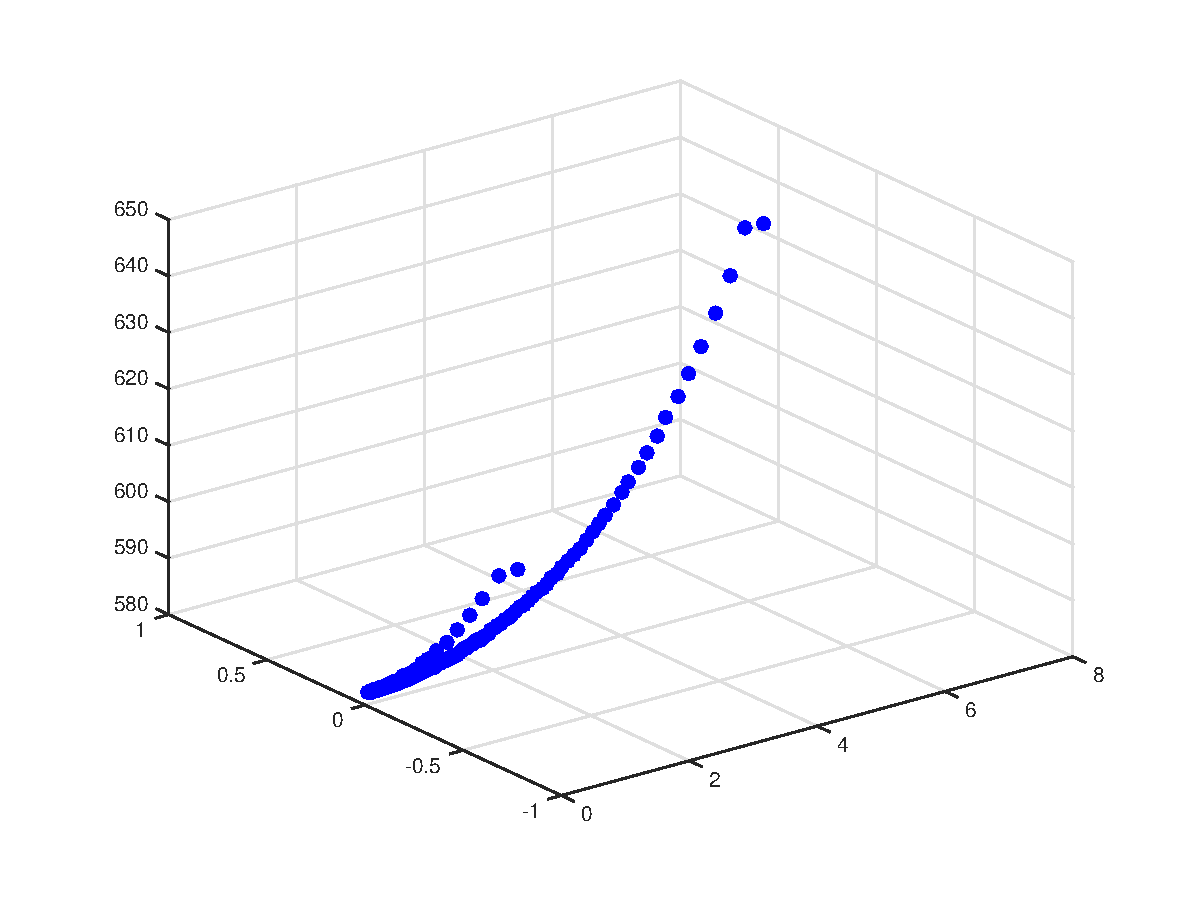
\includegraphics[scale=0.4]{21.eps}
\caption{$K=0.05,0.01, \mathbf{x}_3, \mathbf{x}_4$}
\end{minipage}%
\begin{minipage}[t]{0.5\linewidth}
\centering
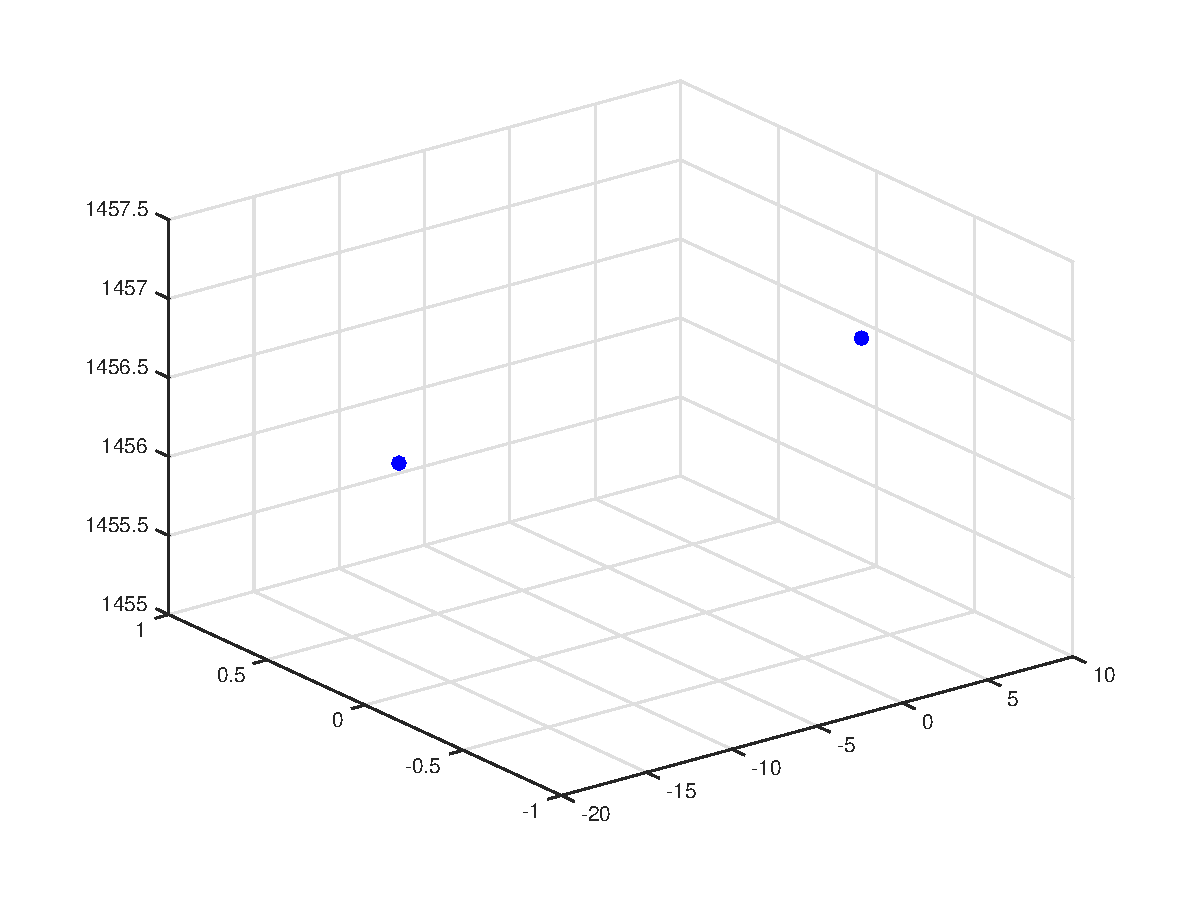
\includegraphics[scale=0.4]{22}
\caption{$K=0.01,\mathbf{x}_5$}
\end{minipage}
\end{figure}
\begin{eqnarray*}
\mathbf{x}_{3} &=& [-0.0580,-0.0624],~ E(\mathbf{x}_1) = 582.0702, ~k_3 = 31 \\
\mathbf{x}_{4} &=& [0.0840,0.0137], ~E(\mathbf{x}_2) = 582.0705, ~k_4 = 172\\
\mathbf{x}_{5} &:& \text{Out-ranged, no feasible result}.
\end{eqnarray*}

\noindent
\textbf{(d)} The plots above shows the trajectory of gradient descending in simulation, with coordinates indicating $x,y$ and $E(\mathbf{x})$. Those visible trajectories represents feasible results found, and scatter points stands for out-ranged results.

To conclude from results in (b) and (c), it is apparent that setting parameters in multiplication of gradient for step-size is not universally available. Modifying $\epsilon$ may optimize obtained feasible results, but remains useless for points near the margins.

Number of steps $k$ increases as parameter $K$ or convergence $\epsilon$ gets smaller, resulting in the total running time tends to be $\mathcal{O}(1/K)$, which is easy to prove.

\newpage
\noindent
\textbf{(e)} Consider a modification in which maximum step size is limited. We set this parameter to 100, 10 and 1, and use the following modification in algorithm, while maintaining $\epsilon = 0.2$.

\begin{algorithm}
\caption{Step size limit}\label{euclid}
\begin{algorithmic}[1]
\State $G \gets \|{\nabla E(\mathbf{x_k})}\| $
\If {$G >= \textit{pmax}$}
\State $\mathbf{p} \gets -(pmax/G) * \nabla E(\mathbf{x_k})$
\Else ~$\mathbf{p} \gets -\nabla E(\mathbf{x_k}) $
\EndIf
\end{algorithmic}
\end{algorithm}

$pmax=100$, initial position $\mathbf{x}_{60} = [-5.4467,-1.2860]$;

$pmax=10$, initial position $\mathbf{x}_{70} = [-5.4816,-6.5858]$, and $\mathbf{x}_{80} = [-9.5 7.5]$

$pmax=1$, initial position $\mathbf{x}_{90} = [1.8979,-4.7558]$.
\begin{figure}[h]
\begin{minipage}[t]{0.5\linewidth}
\centering
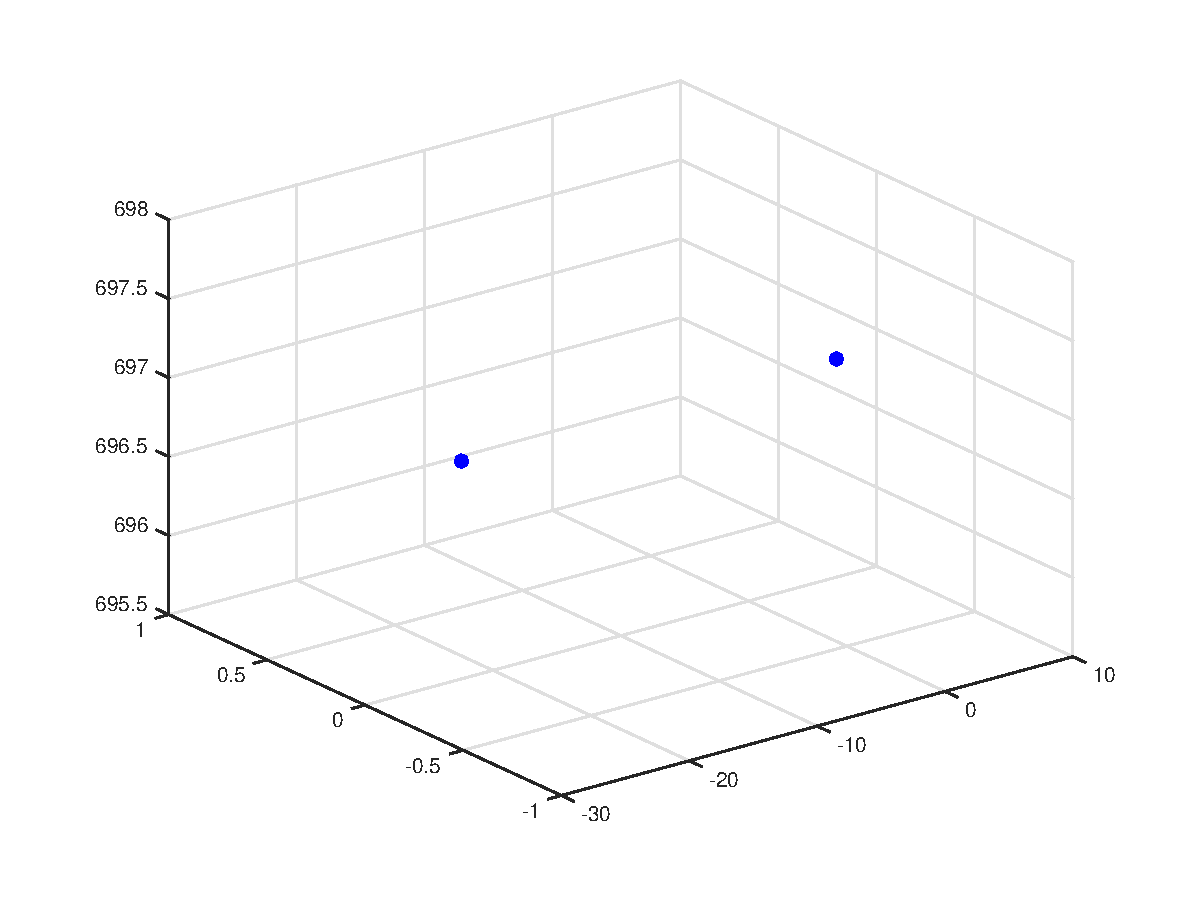
\includegraphics[scale=0.4]{23}
\caption{$pmax=100,\mathbf{x}_6$}
\end{minipage}%
\begin{minipage}[t]{0.5\linewidth}
\centering
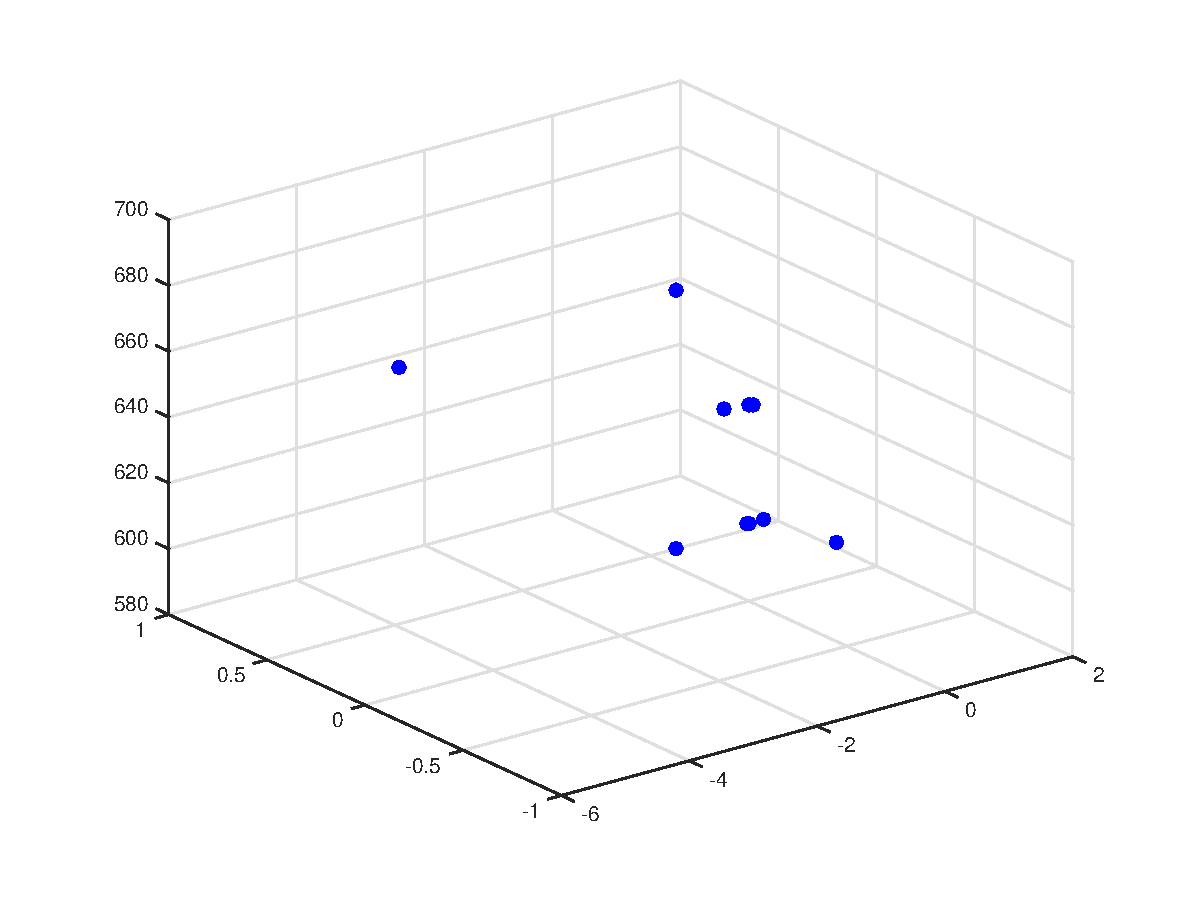
\includegraphics[scale=0.4]{24}
\caption{$pmax=10,\mathbf{x}_7$}
\end{minipage}
\end{figure}

\noindent
As $pmax = 100$, the modification makes no difference. The result remains outside the system, so no feasible results generated.

When $pmax = 10$, the prospective point descends along the gradient to a certain range proportional to $pmax$, and starts \textbf{bouncing back and forth over $O$}, till maxstep is reached (figure 8). There is no feasible local minimum as well. Meanwhile, if the initial point locates near the margins, there is still possibility of yielding out-ranged result, See figure 9.
\begin{figure}[h]
\begin{minipage}[t]{0.5\linewidth}
\centering
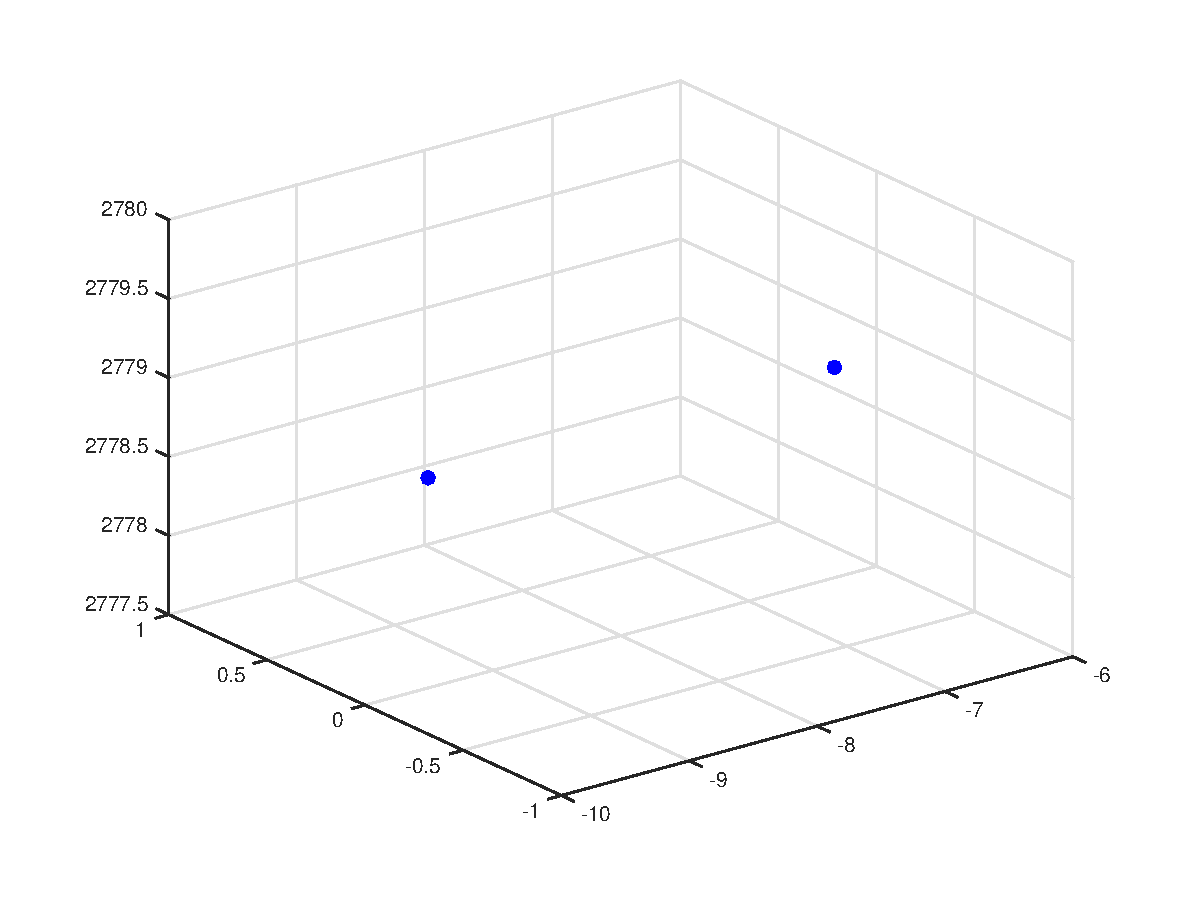
\includegraphics[scale=0.4]{25}
\caption{$pmax=10,\mathbf{x}_8$}
\end{minipage}%
\begin{minipage}[t]{0.5\linewidth}
\centering
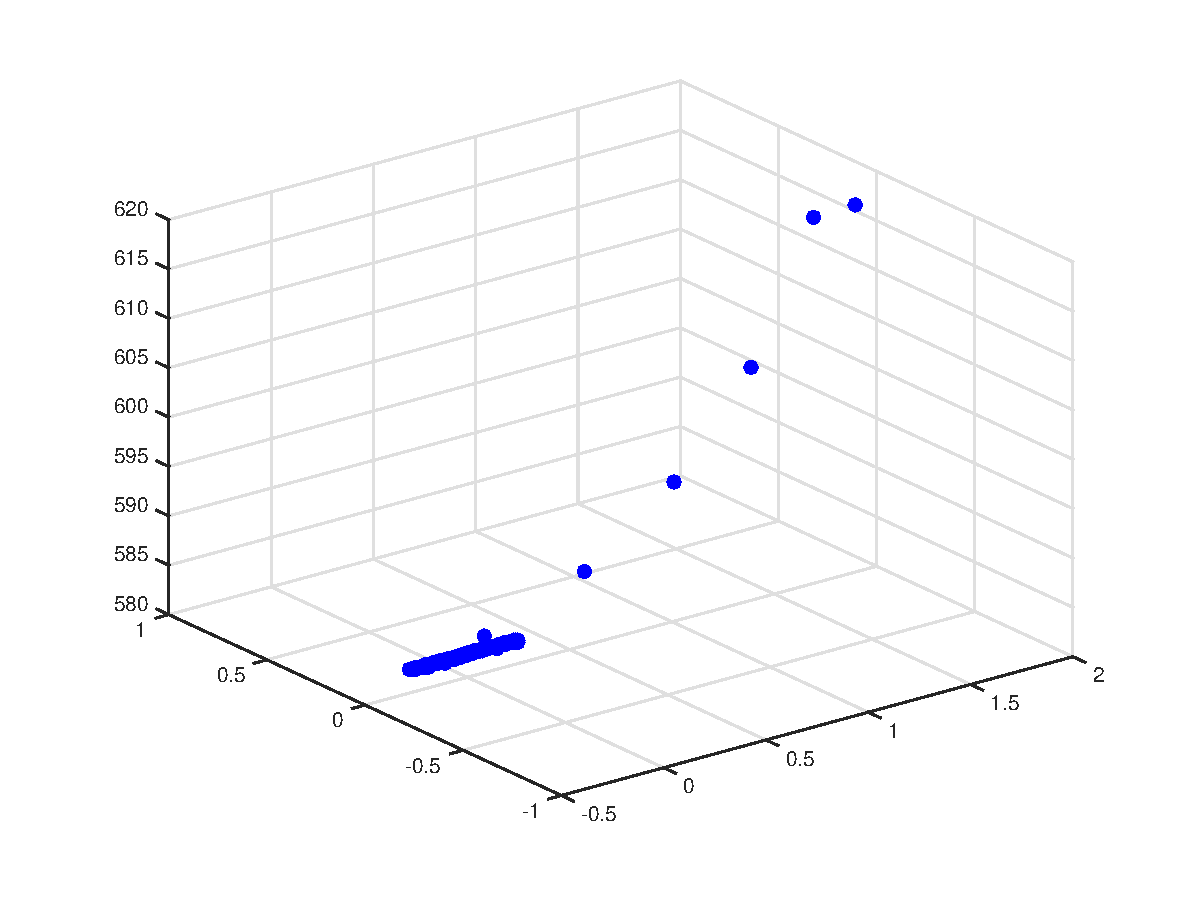
\includegraphics[scale=0.4]{27}
\caption{$pmax=10,\mathbf{x}_9$}
\end{minipage}
\end{figure}

If $pmax=1$, the result ends in bouncing back and forth over $O$ after descending along the gradient, until maxstep is reached, regardless the initial position. See figure 10.

\vspace{3mm}
From simulations with modified algorithm 1, we see that none of the parameters among 100, 10 and 1 could yield a well-behaved feasible local minimum. Large parameters makes no difference, while small parameters of gradients using this algorithm are large enough for the descending point to jump over $O$. This entails another gradient large enough to jump back or form a circulated motion that only stops if maxstep is reached, in which no final minimum occurs. 

So we consider changing the modification by a parameter multiplied to avoid these circular motion. We want every alternative step $\mathbf{p}$ for large $\nabla E(\mathbf{x_k})$ smaller, by setting 
$$\mathbf{p} = -pmax\frac{\nabla E(\mathbf{x_k})}{\|\nabla E(\mathbf{x_k})\|}\cdot G/(1+G)$$
so that $\mathbf{p}$ would not be large enough to form circular motion. Even if the point can jump over $O$, it gets smaller gradient, which leads it to local minimum.
\begin{algorithm}
\caption{Step size limit revised}\label{euclid}
\begin{algorithmic}[2]
\State $G \gets \|{\nabla E(\mathbf{x_k})}\| $
\If {$G >= \textit{pmax}$}
\State $\mathbf{p} \gets -(pmax/G) * \nabla E(\mathbf{x_k}) * G/(1+G)$
\Else ~$\mathbf{p} \gets -\nabla E(\mathbf{x_k}) $
\EndIf
\end{algorithmic}
\end{algorithm}

\noindent
Still the revision makes no difference on $pmax = 100$ and $pmax = 10$ cases. (Fig 11 and 12)

$pmax=100$, initial position $\mathbf{x}'_{0} = [8.5771,4.6066]$;

$pmax=10$, initial position $\mathbf{x}'_{10} = [6.0203,-9.4156]$.
\begin{figure}[h]
\begin{minipage}[t]{0.5\linewidth}
\centering
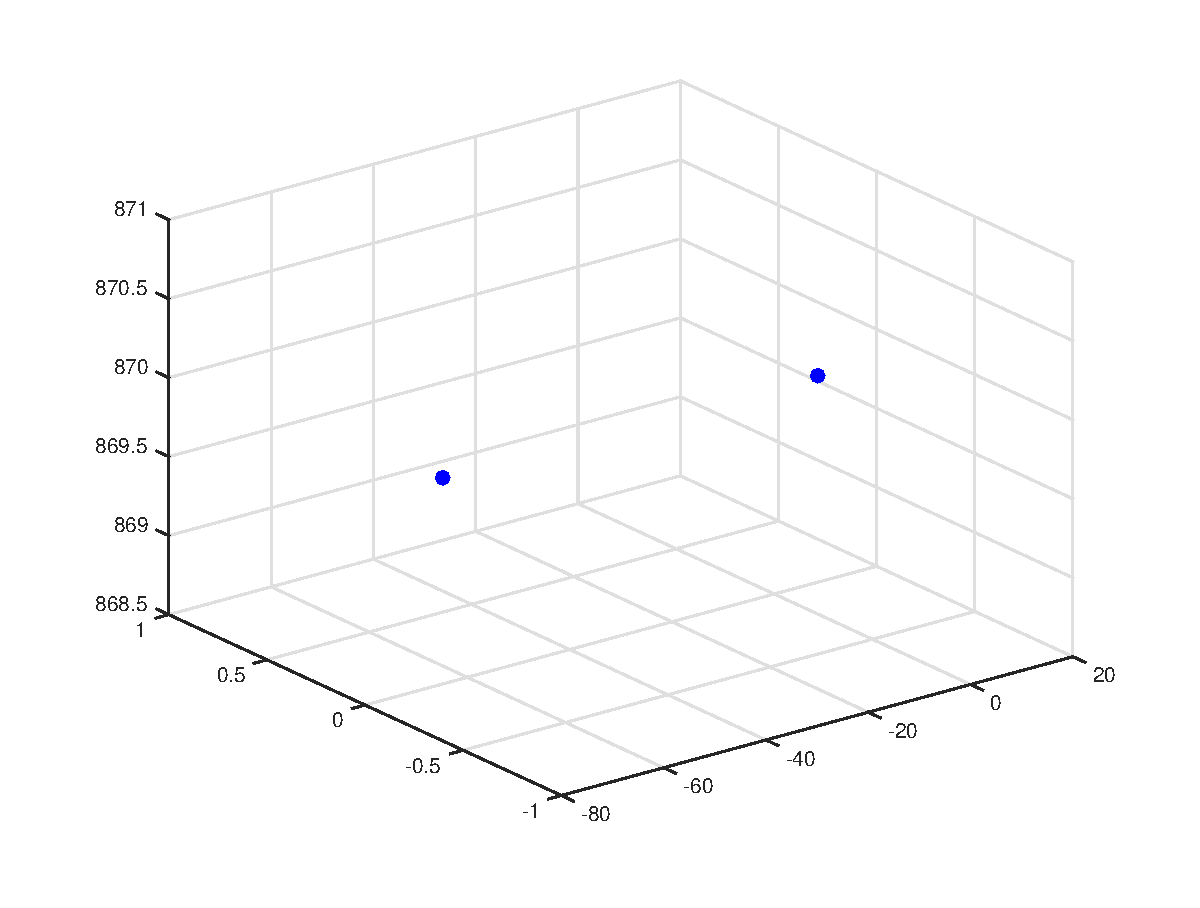
\includegraphics[scale=0.4]{28}
\caption{$pmax=100,\mathbf{x}'$}
\end{minipage}%
\begin{minipage}[t]{0.5\linewidth}
\centering
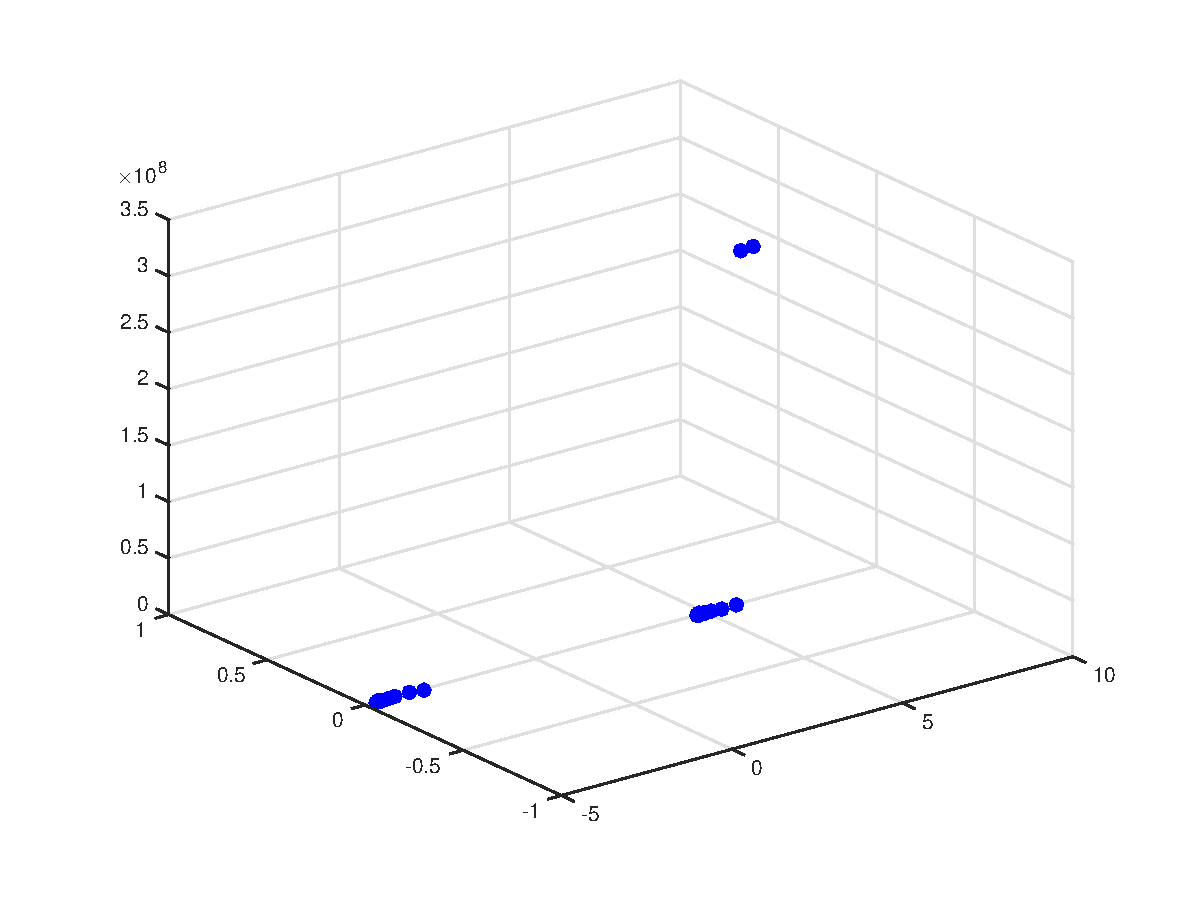
\includegraphics[scale=0.4]{29}
\caption{$pmax=10,\mathbf{x}'_{1}$}
\end{minipage}
\end{figure}

\noindent
But it makes \textbf{every possible starting point at $pmax = 1$ converge to local minimum}. See figure 13 and 14.

$pmax=1$, initial position $\mathbf{x}'_{20} = [-5.2543,-0.8230]$;

$pmax=1$, initial position $\mathbf{x}'_{30} = [-9.2452,7.7034]$.
\begin{figure}[h]
\begin{minipage}[t]{0.5\linewidth}
\centering
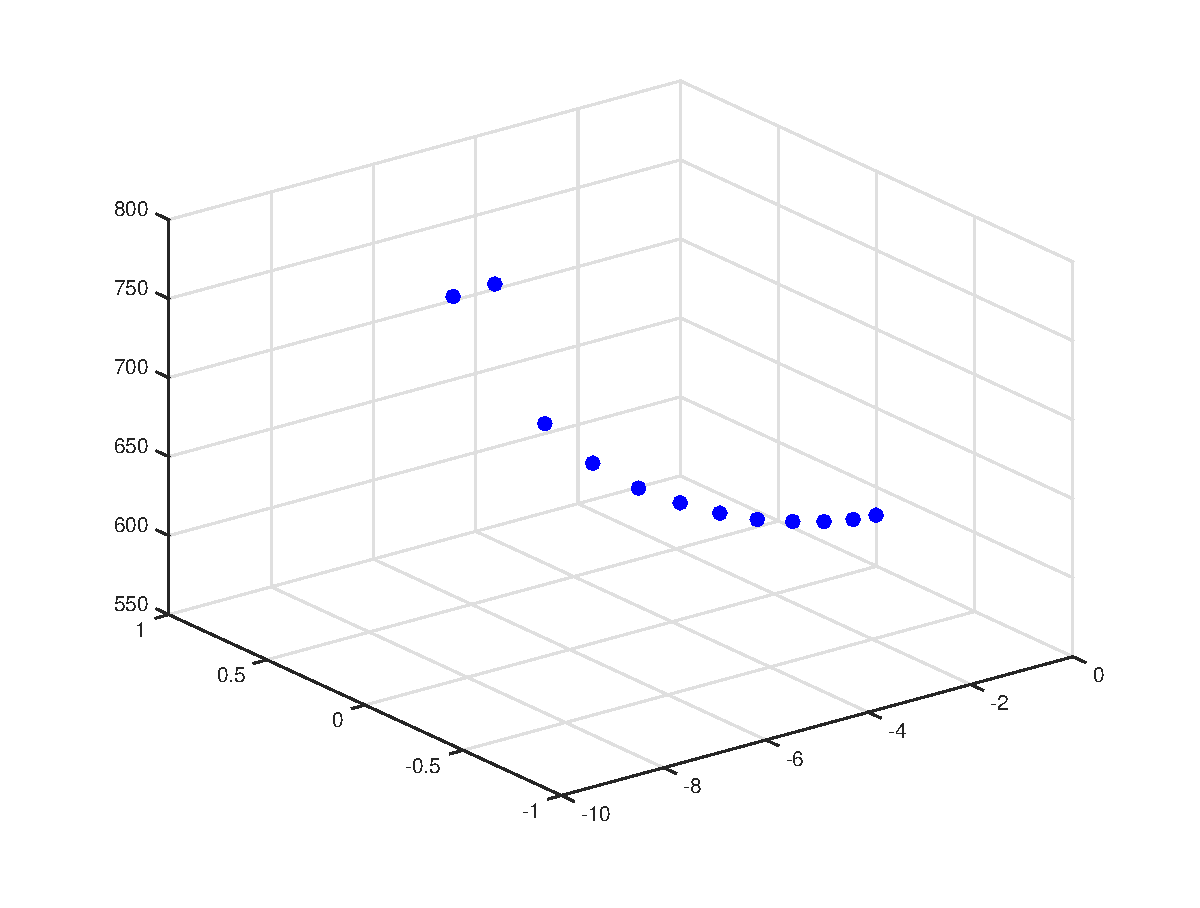
\includegraphics[scale=0.34]{30}
\caption{$pmax=1,\mathbf{x}'_{2}$}
\end{minipage}%
\begin{minipage}[t]{0.5\linewidth}
\centering
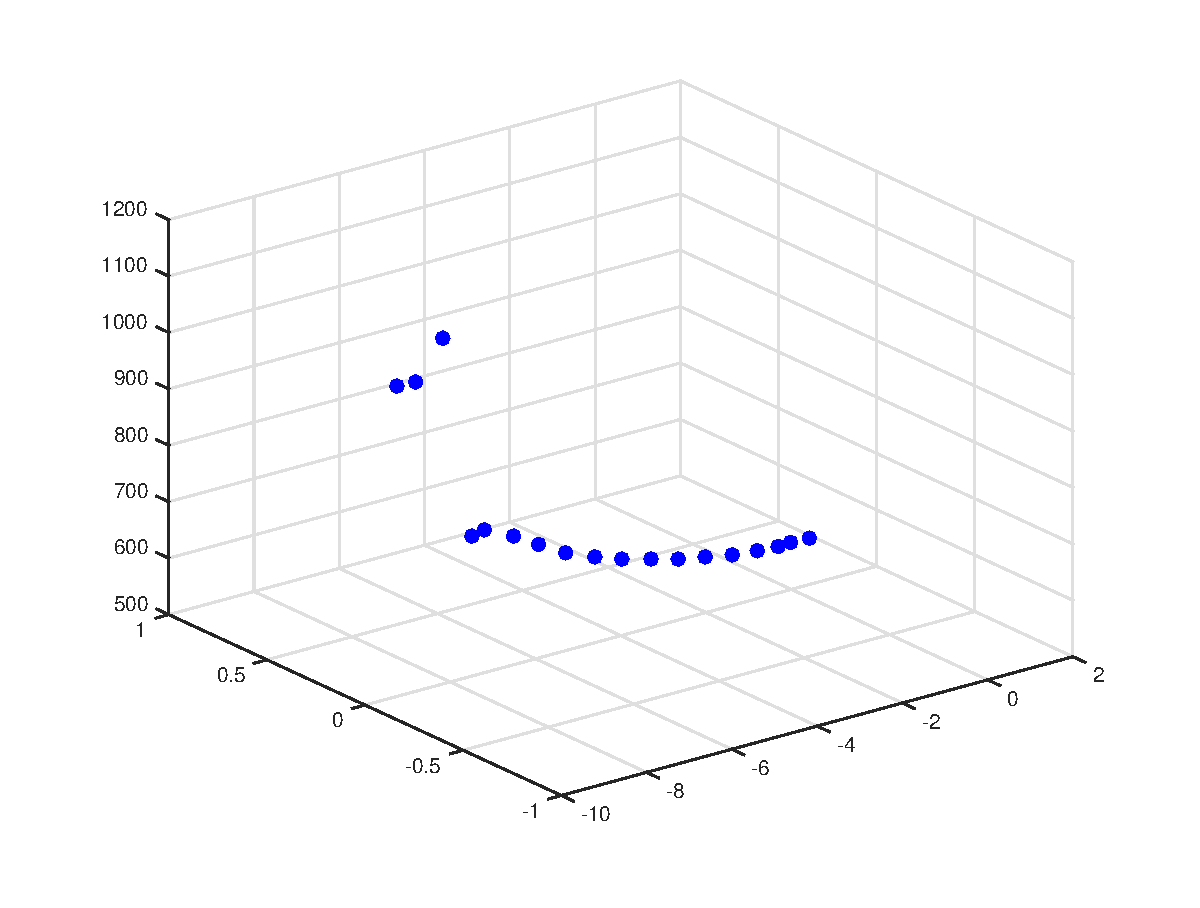
\includegraphics[scale=0.34]{31}
\caption{$pmax=1,\mathbf{x}'_{3}$}
\end{minipage}
\end{figure}
\begin{eqnarray*}
\mathbf{x}'_{2} &=& [-0.0526,-0.013110], ~E(\mathbf{x}'_{2}) = 582.0651, ~k'_2 = 11 \\
\mathbf{x}'_{3} &=& [-0.001057,0.00106], ~E(\mathbf{x}'_{3}) = 582.0617, ~k'_3 = 18.
\end{eqnarray*}

\vspace{3mm}
\noindent
\textbf{(f)} From all above observations, we can conclude
\begin{itemize}
    \item The analytical local/global minimum energy point is origin point $O$.
    \item Setting small parameter before the gradient in $\mathbf{p}$ works well with initial points that are near to $O$, but still yields out-ranged results from marginal points. Besides, the total steps required is $\mathcal{O}(1/K)$, lowering the efficiency of minimum searching at very small $K$'s.
    \item Modifying convergence criterion helps refine those already obtained results (pushing them towards $O$), but also involves more steps.  
    \item Setting maximum step length is an efficient and accurate way if we choose appropriate step size $pmax$, which is, $pmax$ values that are small enough to generate decreasing gradients instead of loops.
\end{itemize}

There are two major types of "badly behaved" minimization paths from the plots what we simulated above.
\begin{itemize}
    \item Out-ranged configurations caused by marginal initial position, as $\mathbf{Xi}_0$ approaches 10. Norm of gradient becomes steeper at margins, so one gradient vector is likely to bring the result directly outside the system. 
    \item Result trail circulating around $O$, initiated by inappropriate maximum step size. This occurs when $\mathbf{p}$ reaches a balance with gradient, where the vector between two sides of $O$ is consistent with gradient of each side. 
\end{itemize}

The out-ranging problem can be diminished by breaking the program if any result outranks the system, while the circulating trails can be detected and discarded through limiting the maximum \# of steps to an acceptable value proportional to the operating time.

\begin{figure}[h]
\begin{minipage}[t]{0.5\linewidth}
\centering
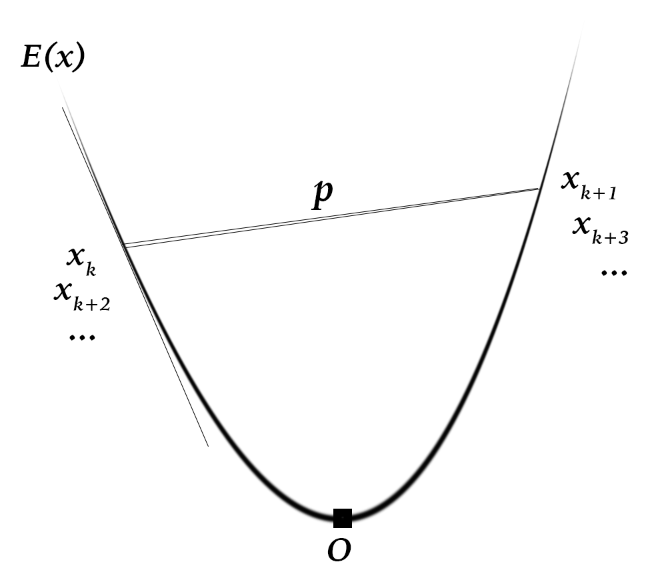
\includegraphics[scale=0.34]{32}
\caption{Bouncing trail}
\end{minipage}%
\begin{minipage}[t]{0.5\linewidth}
\centering
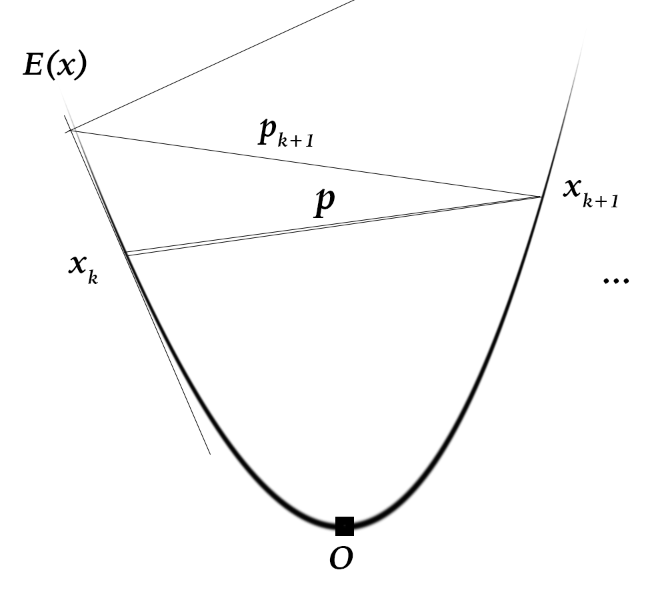
\includegraphics[scale=0.34]{33}
\caption{Out-ranged trail}
\end{minipage}
\end{figure}




\end{document}
